\documentclass[reprint, aps, prl]{revtex4-1}
% \documentclass{article}

\usepackage[margin=0.75in]{geometry}
\usepackage{listings}
\usepackage{graphicx}
\usepackage{fancyhdr}
\usepackage{amssymb}
\usepackage{amsmath}
\usepackage{caption}
\usepackage{subcaption}
\usepackage{enumerate}
\usepackage{subcaption}
\usepackage{textcomp}
\usepackage{placeins}
\usepackage{blindtext}

\usepackage{color}

\begin{document}

\title{Final Report. Laptop Based Doppler Radar }
\author{Albert Wandui \\
\textit{EE 152: High Frequency Systems Lab.}}

\begin{abstract}
We designed and implemented a doppler radar system that was capable of measuring the velocity of a passing car to within 5mph. We implemented our doppler radar system using our own LNA, PA and mixer designs as well as an assymetric Wilkinson and cantennas. The remaining components were purchased from Minicircuits. Here we discuss the design considerations that were taken into account in order to successfully implement the radar system. We measure the performance of each of the subsystems and comment on differences between simulated and measured results. Lastly, we show the results of the radar system in action.
\end{abstract}

\maketitle


% {\let\newpage\relax\maketitle} % Ensures that there is no page break after maketitle



\section*{Introduction}\label{sec:introduction}

We designed and implemented a laptop based Doppler radar system that can be used to measure the velocity of passing objects to within a 40m radius. Doppler radar involves bouncing microwave signals of off a desired target and measuring the induced frequency change due to the motion of the object. Doppler radar finds numerous applications in sounding satellites, aviation, meteorology, radar guns and much more.

The non-relativistic Doppler effect (where the velocity of the object v≪c, the speed of light) can be expressed as 
\begin{equation}
\Delta f= f_{rx}\ -\ f_{tx} = \frac{f_{Tx} \cdot 2 v}{c}.
\end{equation}

Here $f_{rx}$, is the frequency of the received signal and $f_{tx}$ is the transmitted signal. For typical traffic velocities of about 20-45 mph, the Doppler shift ranges from 350-800 Hz. Because the Doppler frequency shift is in the audio range, a laptop sound card with a 16 kbit ADC is well equipped to sample and digitize our desired velocity signal. This was ideal for this project because this reduced the complexity of the receive chain of the radar system significantly.

In this project, in place of more expensive high gain horn antennas that would be typical of scientific or commercial radar instruments, we will design our own cantennas which promised moderate gain at but a fraction of the cost. The cantenna couples power from a quarter wave coax line dipole antenna into a cylindrical waveguide with a diameter d. The waveguide acts to greatly improve the gain of the antenna. For free space wavelength equal to $\lambda$, then the maximum gain for a cantenna is given by $G = \left(\pi d/ \lambda\right)^2$. A waveguide can support many different spatial modes of the electromagnetic field, each of which is an independent solution to the Helmholtz equations in cylindrical coordinates. Each of these modes is characterized by a cutoff frequency below waves in the waveguide are strongly attenuated. This cutoff frequency is determined by the mode number $n, m$ of the waveguide. The $TE_{11}$ mode, which is the fundamental mode of the waveguide and hence the easiest to excite has a cutoff frequency $f_c$ given by the equation

\begin{equation}
    f_c\ =\ c\ \frac{p_{n,m}}{(\pi d)}
\end{equation}

$p_{n,m }$ is the mth root of the first derivative of the nth cylindrical Bessel function. The values of these roots are available in mathematical tables and software. For our purposes, we are interested only in the fundamental with $p_{1,1} = 1.8412$. Figure [\ref{fig:cutoffgain}], overplots the two relevant equations for our antenna design; the cutoff frequency and the gain as a function of the cantenna diameter. In our design, we chose a diameter of 2.7 inches which gives a 12 dBi gain. While the gain is low, the cutoff frequency is conveniently 2.7 GHz, just above the 2.4 GHz ISM band in which wifi, Bluetooth and other short range low power transmission systems are allocated. Such signals would cause high levels of interference rapidly degrading our measured signals. In practice, we expected our cantennas to achieve much lower gains and so we designed our system to work effectively even with cantenna gains as low as 3 dB.

\begin{figure}[!htbp]
    \centering
    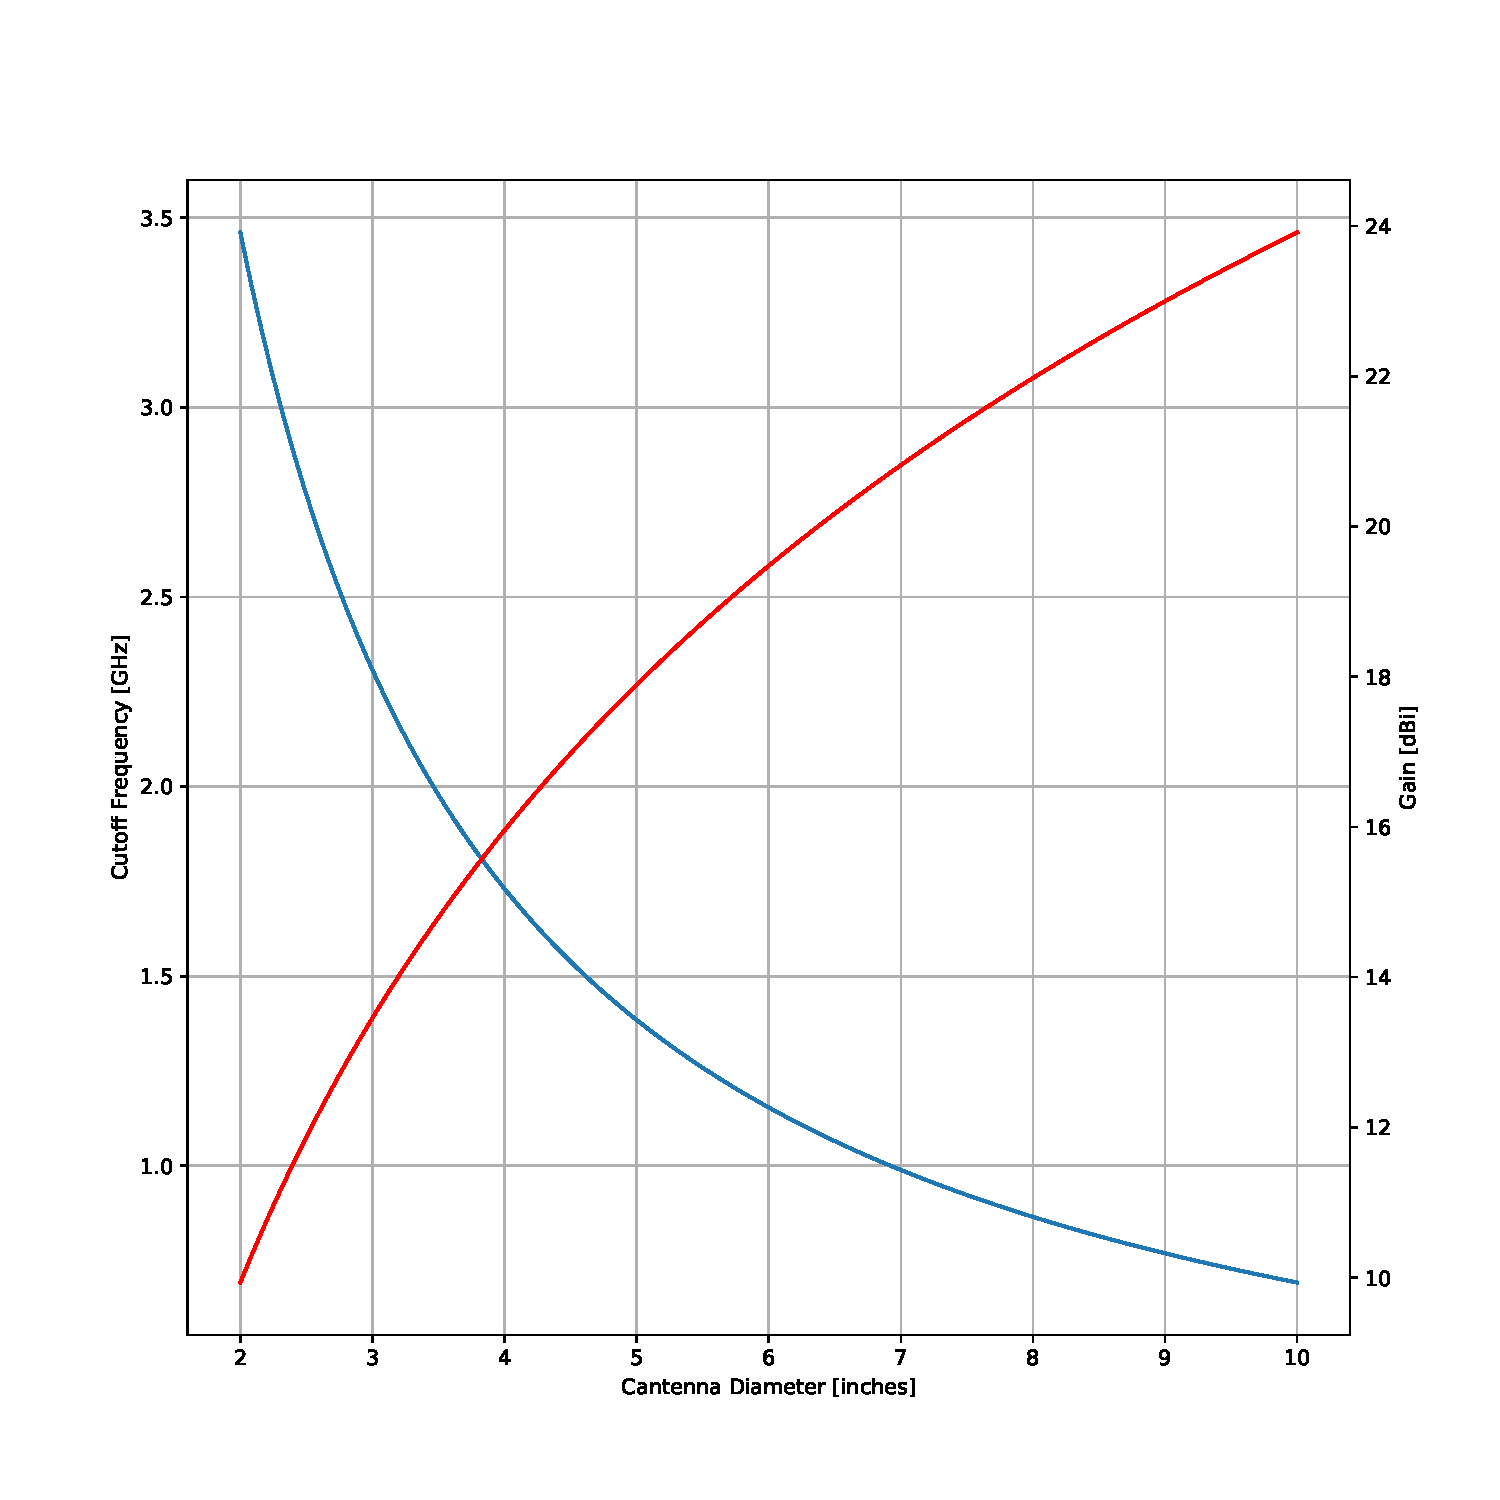
\includegraphics[scale=0.35]{cantenna.pdf}
    \caption{The cutoff frequency and gain as a function of diameter for a cantenna.}
    \label{fig:cutoffgain}
\end{figure}

Using the antenna equations and given the transmitted power $P_{tx}$, we can calculate the power in the receiver, $P_{rx}$. The ability of a target to be detectable by the radar system is encoded in the radar cross section of the target σ. The radar cross section defined as the ratio between the scattered power and the incident power flux. For a target at a distance R from the antenna with a gain G in the direction of the target, the power flux is given by 

\begin{equation}
\frac{P_{tx} G}{4 \pi R^2}.
\end{equation}

The target (we assume) scatters the radiation isotropically in all directions and thus acts as an antenna of its own. The receiver sees the radiation from this antenna and we can compute the power at the receiver using the Friis transmission equation as 

\begin{equation}
P_{rx} = \left(\frac{P_{tx} G}{4 \pi R^2} \sigma \right) \cdot \left(G \frac{\lambda^2}{4 \pi R^2} \right) \cdot F^4
\end{equation}

The first term in brackets, is the power radiated by the target back towards the receiver. The second term is the effective area of the receiving antenna while the factor F is the pattern propagation factor. F encapsulates higher order effects such as diffraction, further scattering and multipath transmission between the source and the target. The power measured at the receiver has a strong $1/R^4$ dependence and hence is very sensitive to changes in the transmitted power, gain or pattern propagation.

\section{Design Considerations and Description}
For a radar system, noise considerations strongly constrain the design of the system. To goal of detecting the doppler shift with a desired signal to noise ratio (SNR), sets a sharp lower bound on the amount of power that must be collected by the receiving cantenna. This in turn constrains the amount of power that must be transmitted. The transmit chain of the radar must have enough gain to send adequate signal out towards the target. In addition, it sets a limit on the range of the radar system, that is the farthest distance that the target could be, away from the radar, for a sufficiently large signal to be detected at the receiver. In the design of the receive chain, care must also be taken to ensure that the noise contributions due to the elements in the chain do not load the signal being received severely degrading the SNR. A schematic of the design of the doppler radar system is shown in figure [\ref{fig:radarschematic}]

At the receiving cantenna, our goal was to measure the doppler signal with an SNR of 2, achieve a system noise temperature of 300 K assuming an RF bandwidth of say 1 GHz (our cantenna being well matched to frequencies in this range around the design frequency of 5.9 GHz). The expected noise level at the receiver is then given by $k T B = -84$ dBm. A signal with an SNR of 2 would be imply that $P_{rx} = -81$ dBm. For a car, we expect a radar cross-section of  3 square meters. Using the radar equation with F = 1 and for a transmit frequency of 5.9GHz, we can find an expression for the range of our radar system. For the transmit chain of the radar, we used Minicircuits components; the VCO ZX95-5776-S+ which from the datasheet, sources 1.5dBm power and a ZX60-V63+ amplifier with a 15.4 dB gain 6 GHz. This amplifier has its 1-dB compression point at an output power of 12dBm. This necessitates the use of a 5 dB attenuator between the VCO and the amplifier. The power divider stage is placed right after the first amplifier. We designed the unbalanced power divider stage to have a 1 dB loss to the transmit cantenna and a 5 dB loss to the mixer. We have 11 dBm of power in the transmit chain right after the power divider. We add a second amplifier of the same make as the first bringing the power transmitted to the antenna to 26.5 dBm. In actuality, the second amplifier is well in its saturation level since the output power is much higher than 12 dBm. We take additional hits from cable losses which we estimated at being about 2dB. Using a final estimate of 24 dBm power, which is approximately 250 mW, into the transmit cantenna, we can back out the expected range of the radar system from the radar equation. We will use a modest estimate of the antenna gain of about 3 dB. This was informed by the lab measurements of a larger 4" diameter can that had a 5 dB gain which was much lower than the expected 20dB gain. This gives a range of about 27m. For more optimistic cantenna gain estimates at about 5 dB the range increases to 34m. Higher gain could be obtained by using a much wider can for the cantennas. This comes at a price; the larger diameter suppresses the cutoff frequency of the fundamental mode below 2.4 GHz. At this frequency is the ISM band in which wifi works. This exposes the radar system to much higher levels of unwanted background and would necessitate a bandpass filter be introduced in the receive chain to suppress signals in this band. This comes at the cost of worse noise performance due to the noise of the bandpass filter introduced.

The key sources of noise in our receive chain are the mixer and the amplifiers. In addition, we accounted for the additional noise due to losses in the cable and suboptimal connections between the different microwave components. The noise in the receiver chain referred to the cantenna can be calculated using the Friis noise equation. If the noise temperature of the ith subsytem is given by $T_i$ and the gain by $G_i$, then the total noise temperature of the system, $T_{sys}$, can be calculated as

\begin{equation}
T_{sys} = T_1 + \frac{T_2}{G_1} + \frac{T_3}{G_1 \cdot G_2}.
\end{equation}

The first component in the receive path is the cable connecting the cantenna to the amplifier stage. The noise temperature of the cable is related to the attenuation A of the cable and the physical temperature of the cable by the equation $T_1 = (A - 1) T_{phys}$. For $T_{phys} = 290 K$ and cable losses of about 1-2dB, the noise temperature of the cable ranges between 75-170K. With about 20dB gain in the LNA system. Optimally, we expected the mixer to have a conversion loss of 8dB. However, from previous lab measurements, we noted that the conversion loss was expected to increase for very low IF frequencies below about 1 kHz. From in class discussions, we expected the mixer noise temperature to be about 3000K. However, due to the large gain of the amplifier stage, the noise contribution of the mixer stage is significantly reduced. This means that for a system noise temperature of about 300K, the LNA targeted noise temperature is about 150K. With the noise requirements of the receiver satisfied, we turn to the gain requirements of the receive chain. The gain requirements are set by the dynamic range of the ADC on the sound card. We require enough gain to be able to resolve the signal but not enough to cause the ADC to clip at the maximum value. For a 10V, 16 bit ADC, the minimum resolvable voltage is given by $10 V/ 2^{16} \approx 150 \mu V$. With a $200 \Omega$ resistor at the DAC this translates to -69 dBm power into the ADC. Taking an 8 dB conversion loss of the mixer (as discussed earlier, we actually expect much higher conversion loss), we have -61 dBm of power at the end of the low noise amplification stage. This implies that our LNA stage should have a total gain of about 20 dB. We combined our LNA and PA amplifiers from previous labs to obtain a low noise amplification stage with a total simulated gain of about 27 dB. The limited dynamic range of the ADC makes our signal clip for targets that are too close to the radar system.

\begin{figure}[!htbp]
    \centering
    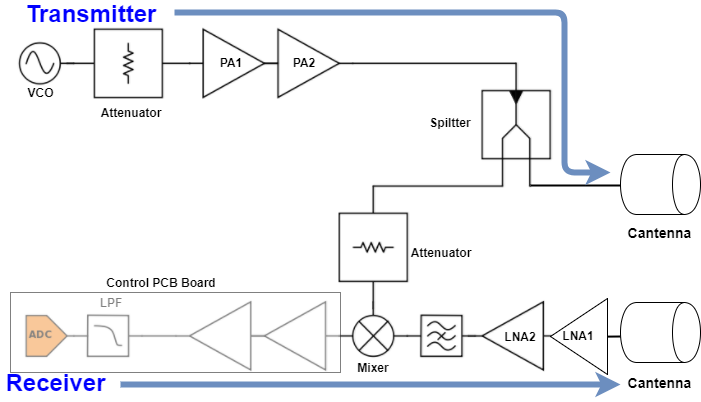
\includegraphics[scale=0.35]{radar_schematic}
    \caption{Schematic of the Radar System.}
    \label{fig:radarschematic}
\end{figure}

\section*{Circuit Fabrication}

- Talk about Cantenna assembly. Drilled holes with the help of the instructors. Hole marked at 13mm - quarter wavelength distance from the back short made by the back of the can. To make the central dipole, started with a longer section and while measuring the return loss of the cantenna, trimmed the length of the antenna wire until the return loss was minimized. The figure [\ref{fig:cantenna}] is a photo of one of the both the cantennas with the dipole conductor visible in the cantenna on the left.

\begin{figure}[!htbp]
    \centering
    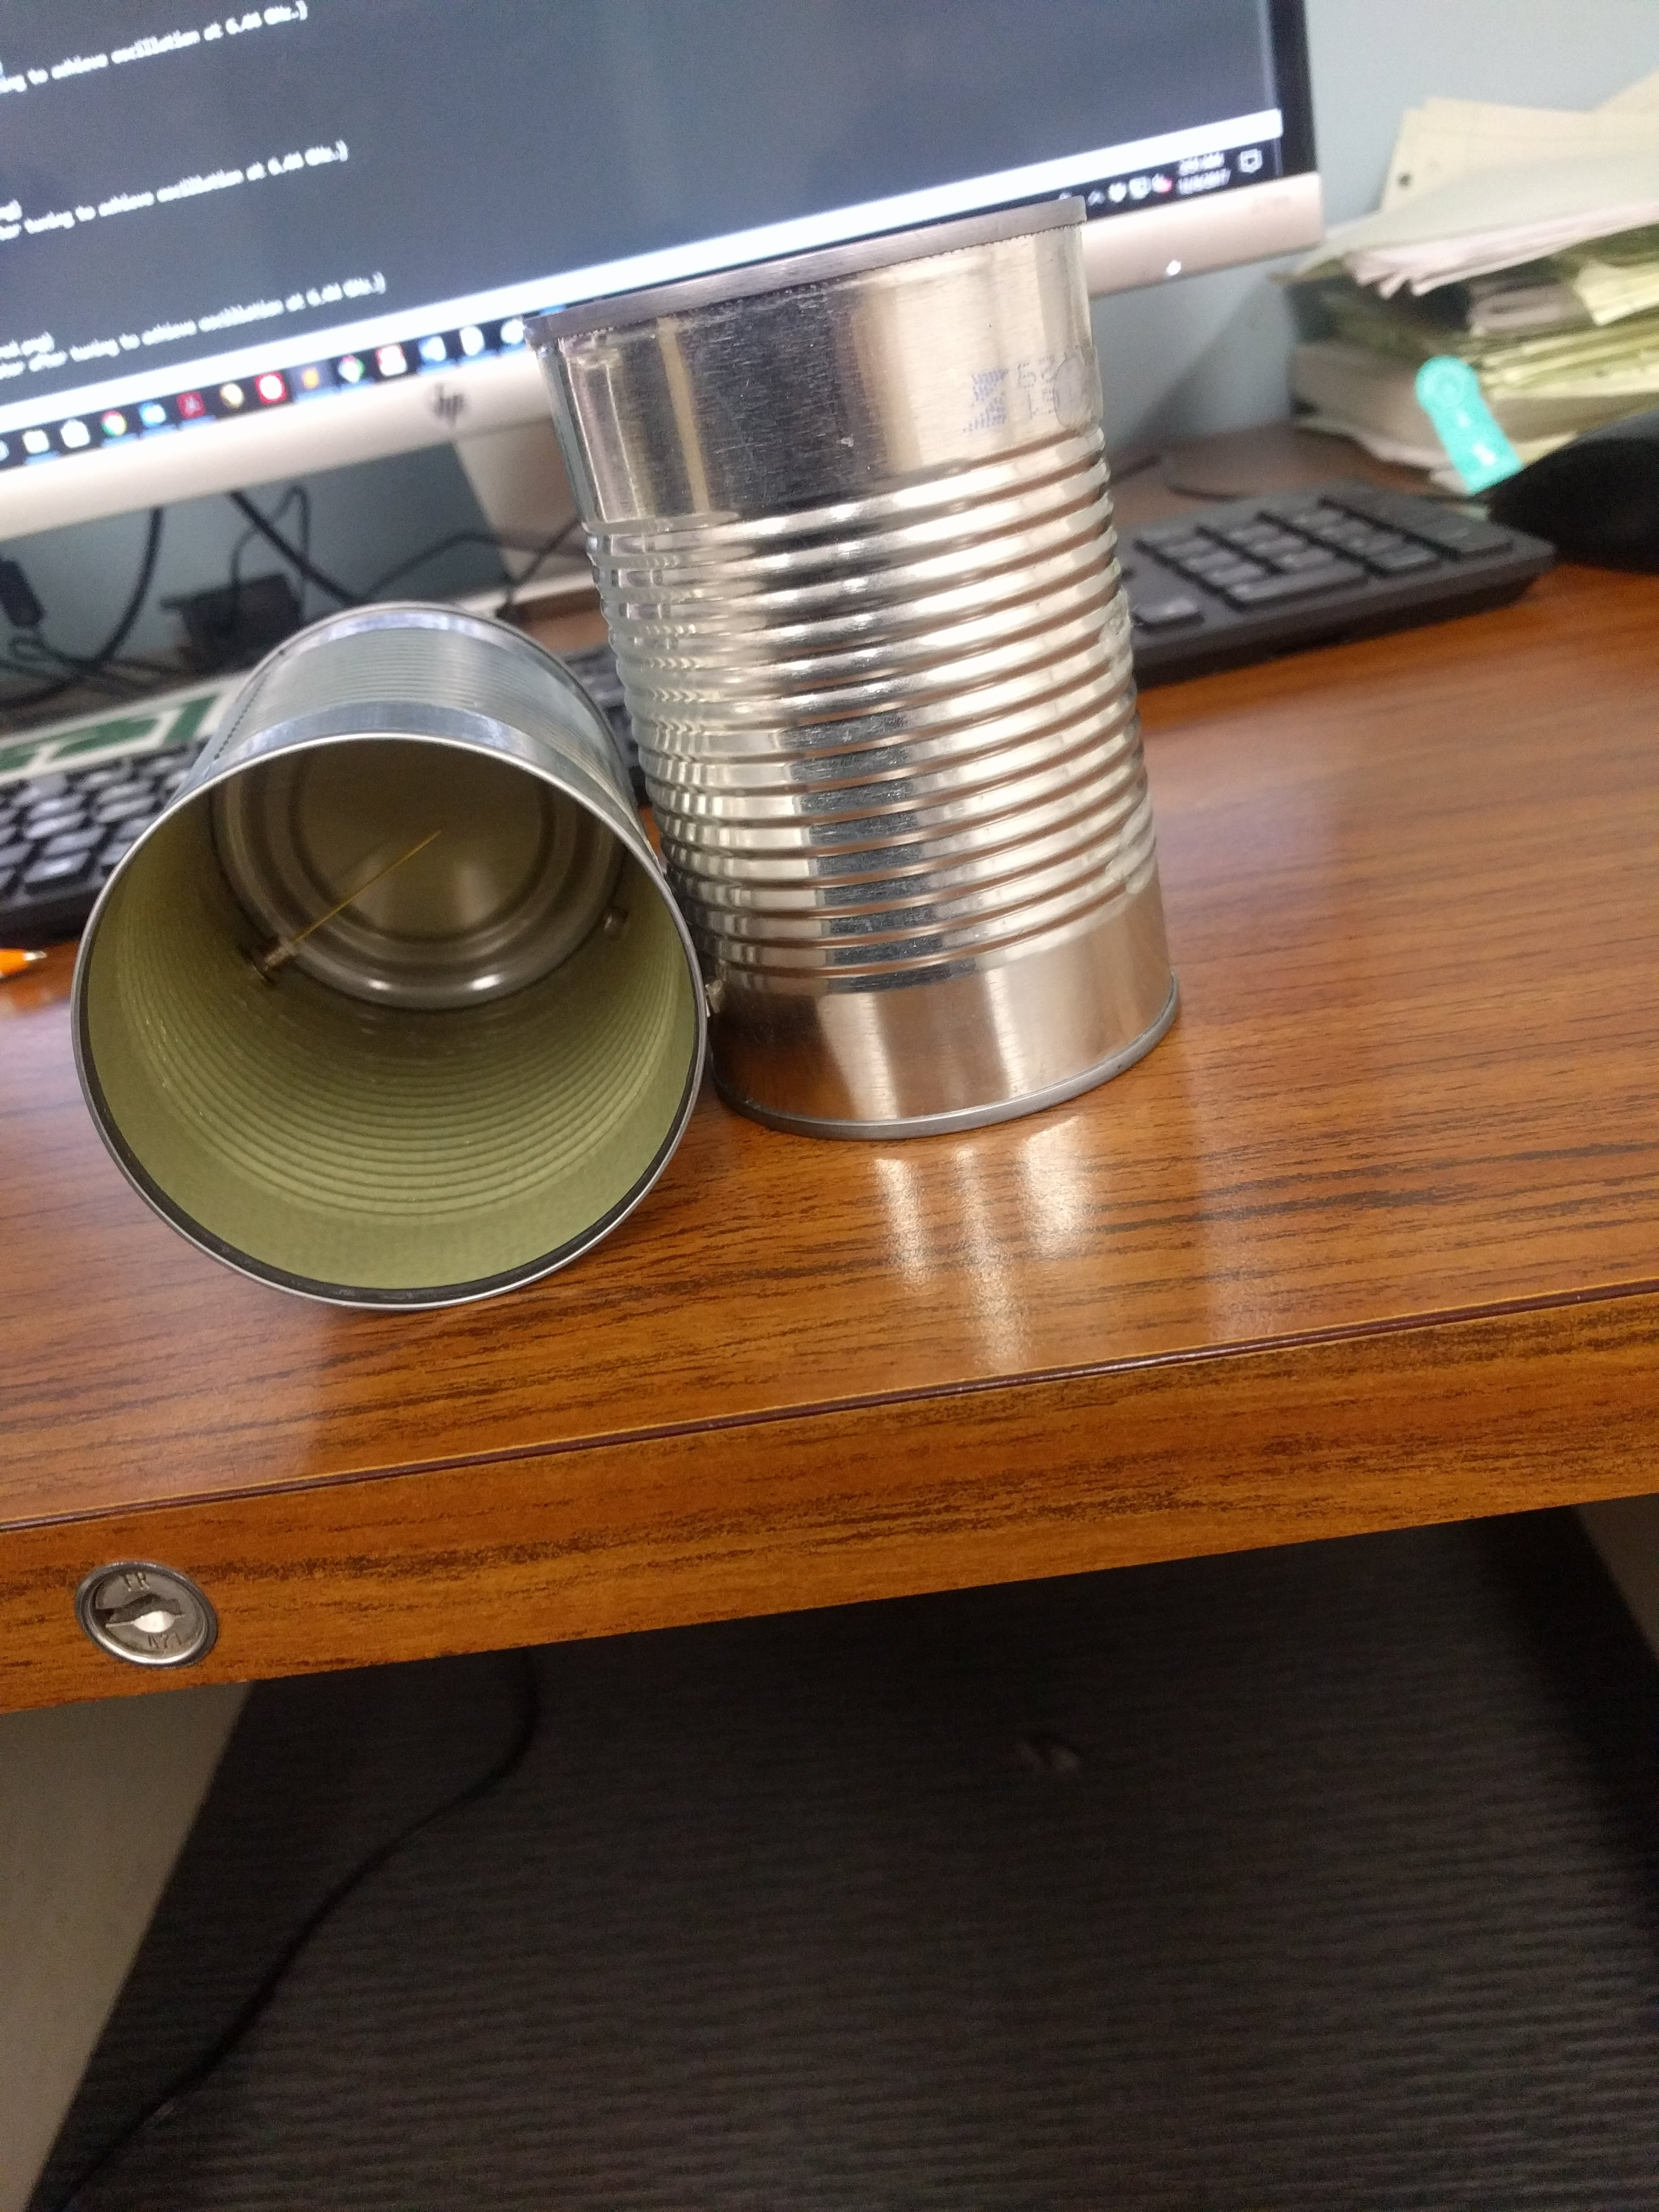
\includegraphics[scale=0.05]{Photos/cantenna.jpg}
    \caption{A photograph of the fabricated cantenna.}
    \label{fig:cantenna}
\end{figure}

We relied heavily on already implemented circuits from our previous labs to minimize the time it took to design new components. The only new design that we implemented was the assymmetric Wilkinson for unbalanced power division. The assymmetric Wilkinson uses transmission lines of two different characteristic impedances that realize the desired power split ratio. A resistor is used to provide isolation between the two outputs as in the balanced Wilkinson case. The schematic of our implemented design for the unbalanced Wilkinson is shown in figure 
[\ref{fig:AsWilkSchematic}]. The simulated performance of the power splitter is shown in figure [\ref{fig:AsWilkParams}]. The actual fabricated device is also shown in figure [\ref{fig:unbalanced}].

\begin{figure*}[!htbp]
    \centering
    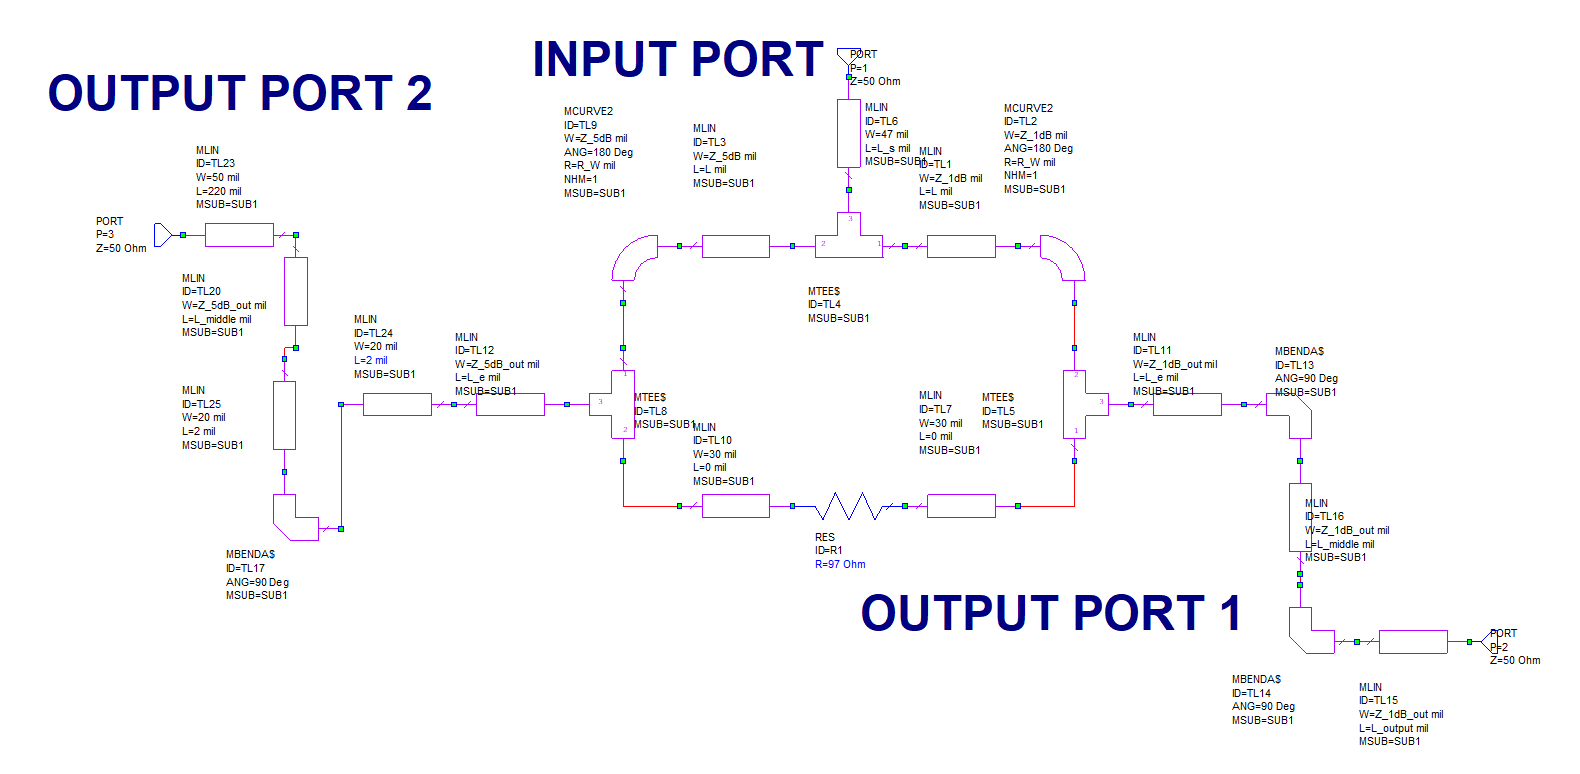
\includegraphics[scale=0.35]{Unbalanced_Wilkinson_Schematic.png}
    \caption{Schematic of the Unbalanced Power Splitter.}
    \label{fig:AsWilkSchematic}
\end{figure*}

\begin{figure}[!htbp]
    \centering
    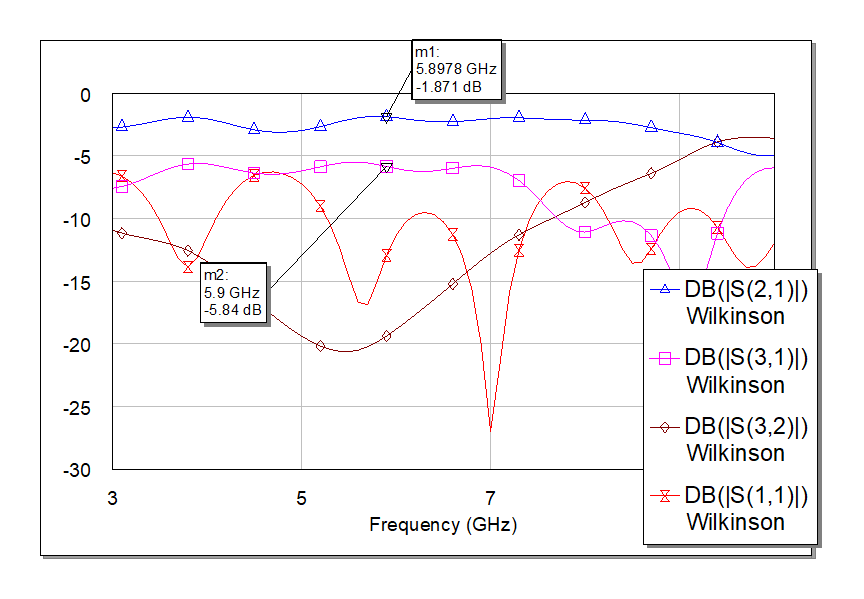
\includegraphics[scale=0.35]{Unbalanced_Wilkinson_params.png}
    \caption{Simulated S parameters of the assymmetric Wilkinson.}
    \label{fig:AsWilkParams}
\end{figure}

\begin{figure}[!htbp]
    \centering
    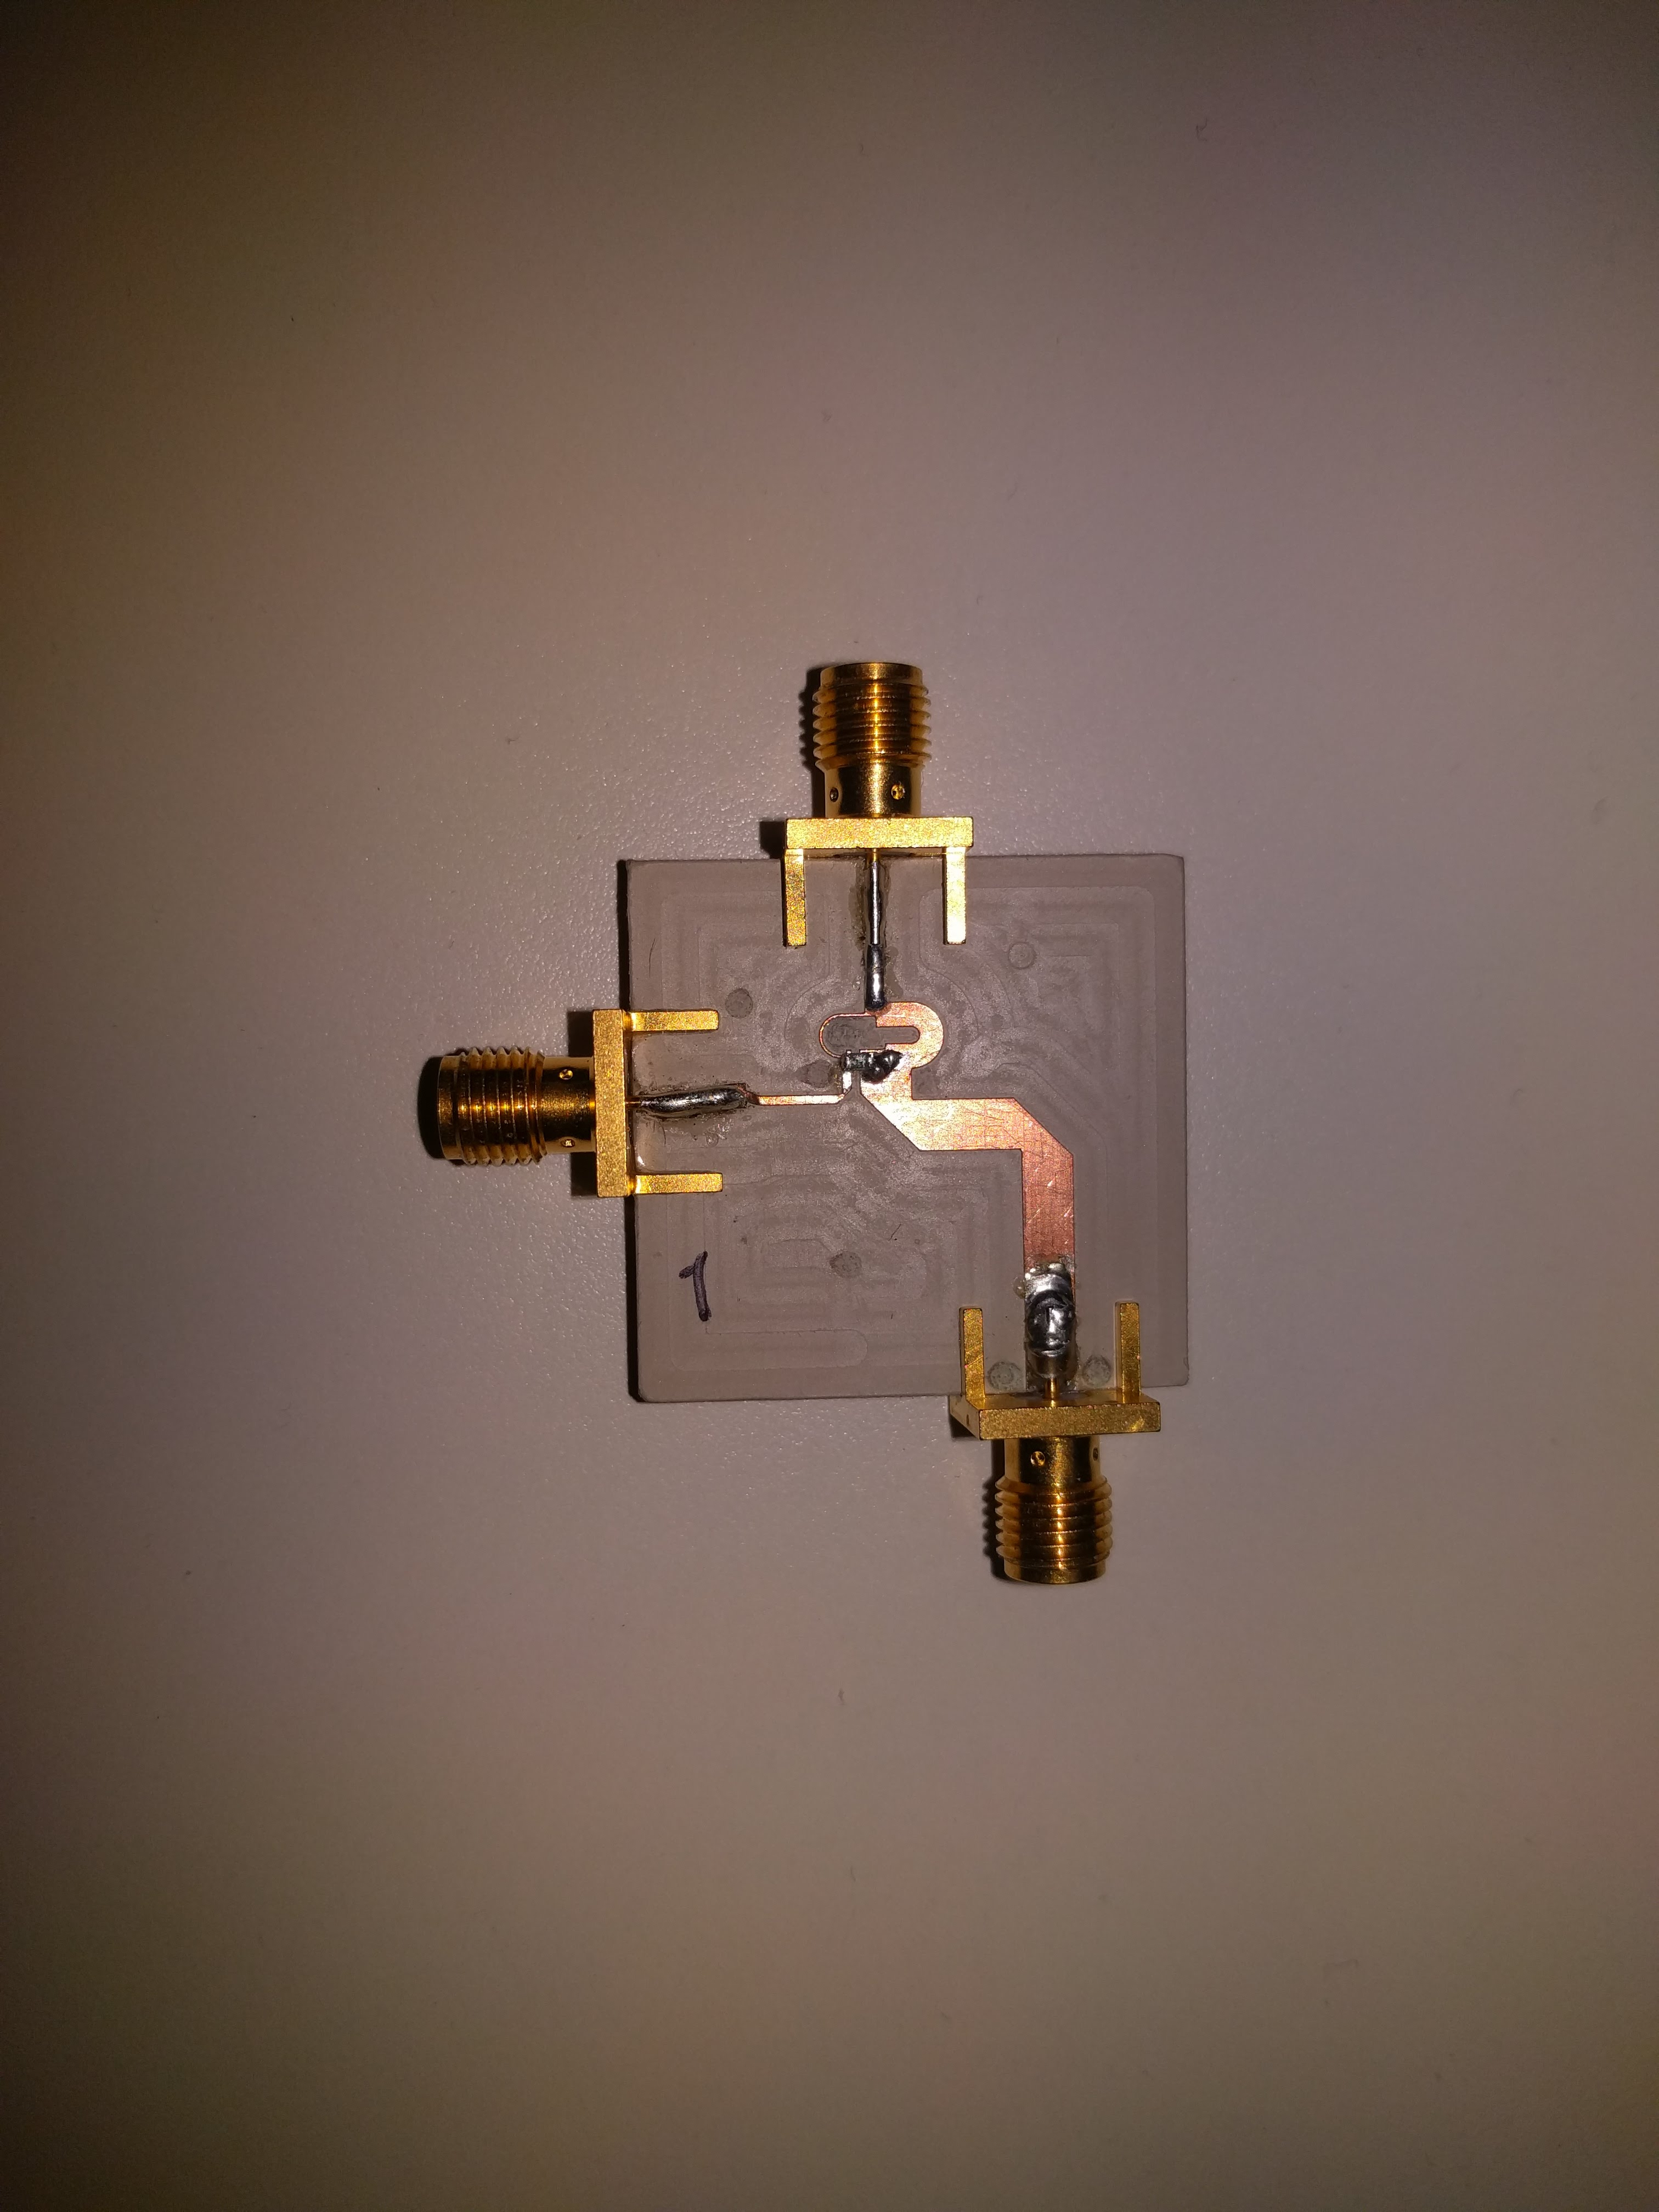
\includegraphics[scale=0.05]{Photos/unbalanced.jpg}
    \caption{A photograph of the fabricated assymmetric Wilkinson.}
    \label{fig:unbalanced}
\end{figure}

To achieve much higher isolation between the RF and LO ports of our mixer, we redesigned our mixer circuit for the radar project. However, the new design had about 4 dB higher conversion loss than our design from lab 4. We decided then, to simply use our mixer design from lab 4 because it's performance was already very well characterized and importantly, it functioned well even for very low IF frequencies in the low kHz range. The actual fabricated device is also shown in figure [\ref{fig:mixer}]. The mixer performance is further discussed in the subcomponent performance section.

\begin{figure}[!htbp]
    \centering
    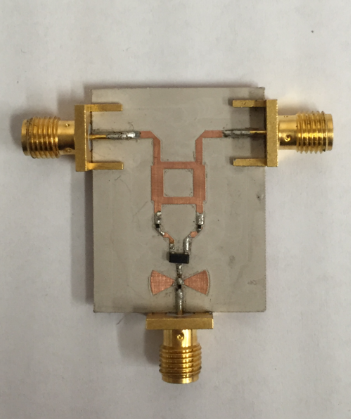
\includegraphics[scale=0.05]{Photos/mixer.jpg}
    \caption{A photograph of the fabricated mixer.}
    \label{fig:mixer}
\end{figure}

For the LNA and PA, we again relied on our designs from the previous labs. We used a combination of the two to provide the high gain and good noise performance that we needed right after the Rx antenna. The figure [\ref{fig:amplifier}] is a photo of one of the amplifiers.
\begin{figure}[!htbp]
    \centering
    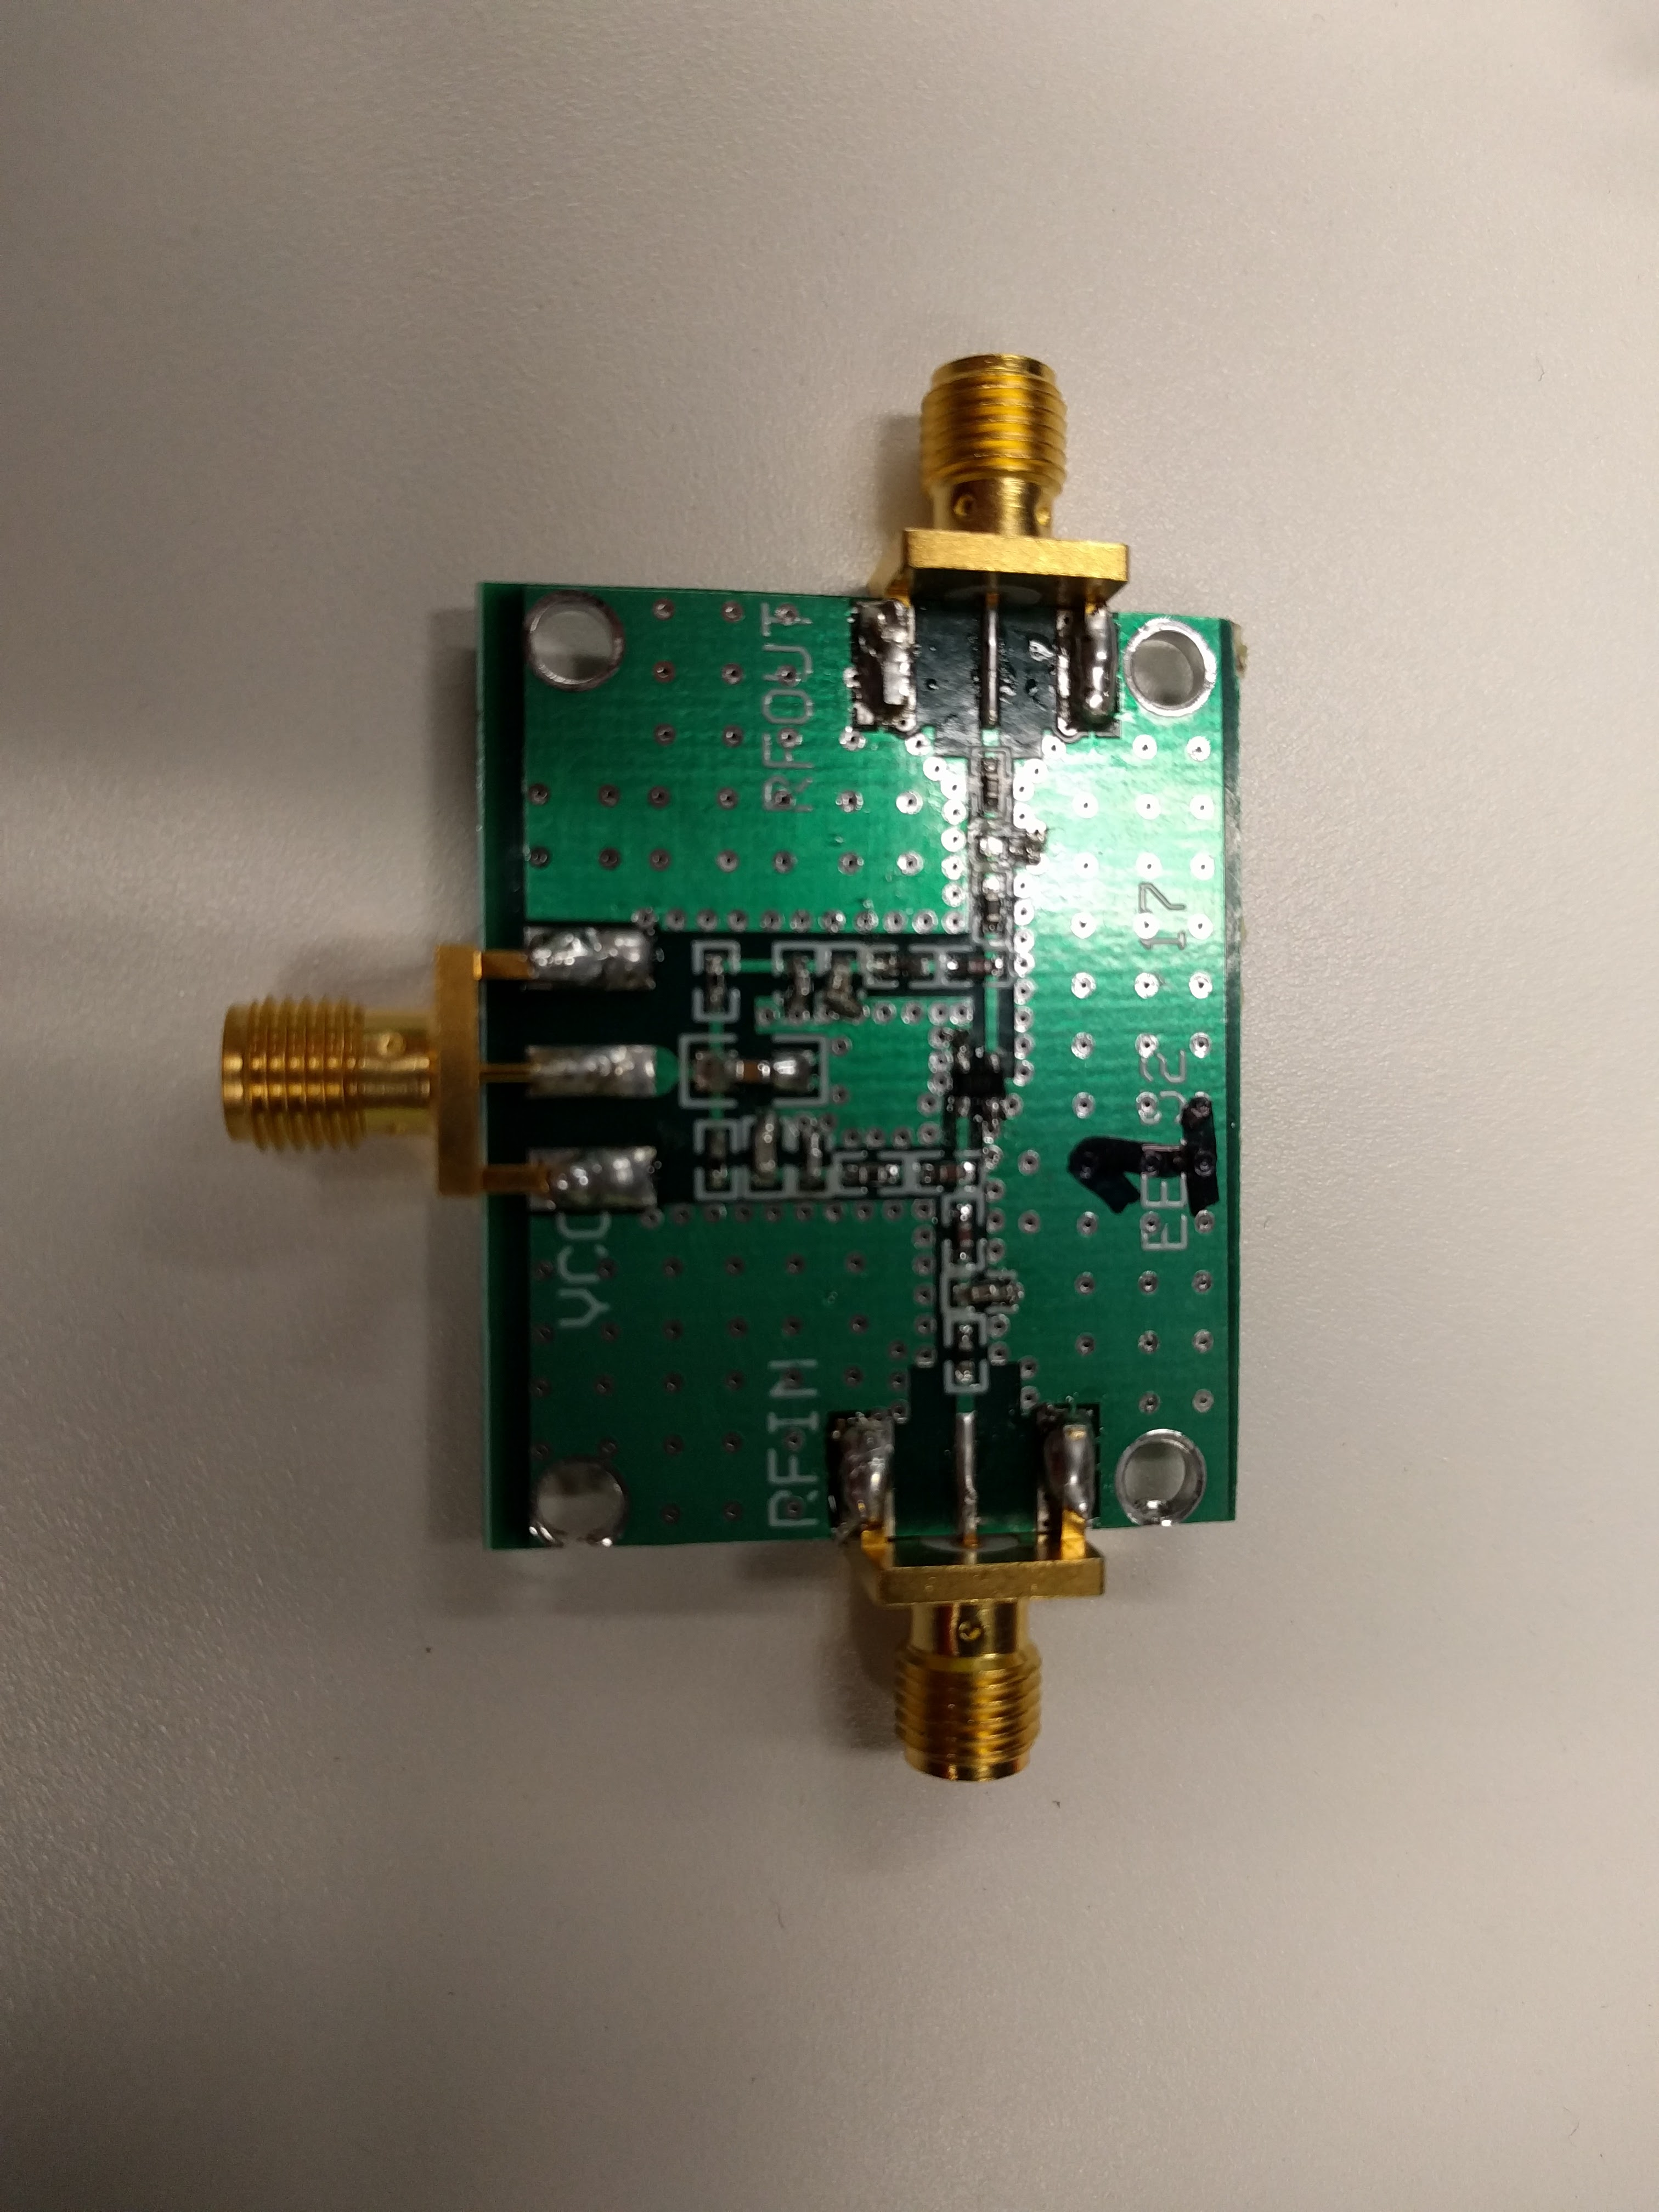
\includegraphics[scale=0.05]{Photos/amplifier.jpg}
    \caption{A photograph of the fabricated amplifier.}
    \label{fig:amplifier}
\end{figure}


\section*{Subcomponent Performance}

- As mentioned, measured the S11 of the cantenna. Worked to minimize it by adjusting the length of the dipole conductor through the wall of the can. Figure [\ref{fig:cantennaS11}] shows the results of these measurements.

\begin{figure}[!htbp]
    \centering
    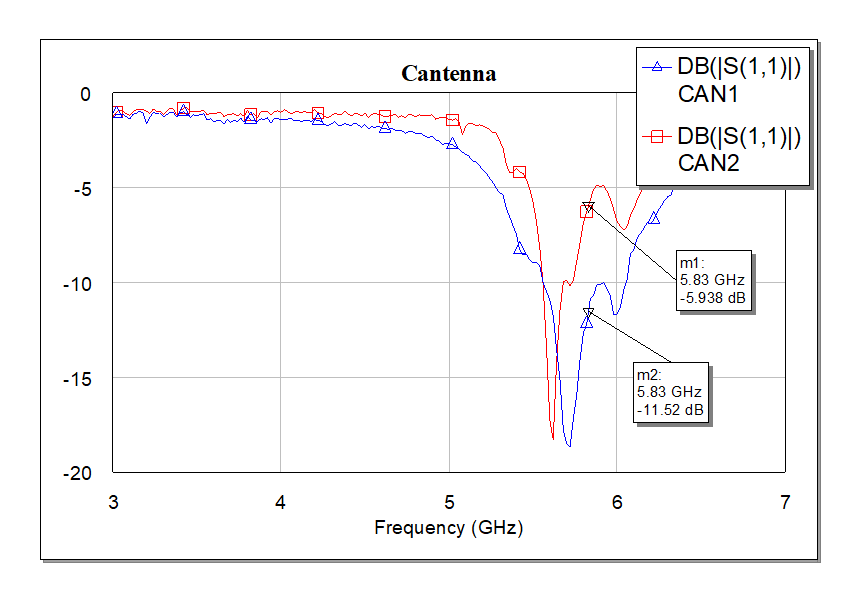
\includegraphics[scale=0.35]{Cantenna_S11.png}
    \caption{S11 for the cantennas.}
    \label{fig:cantennaS11}
\end{figure}

Mixer Measurements.
- Measured isolation at the IF


\begin{figure}[!htbp]
    \centering
    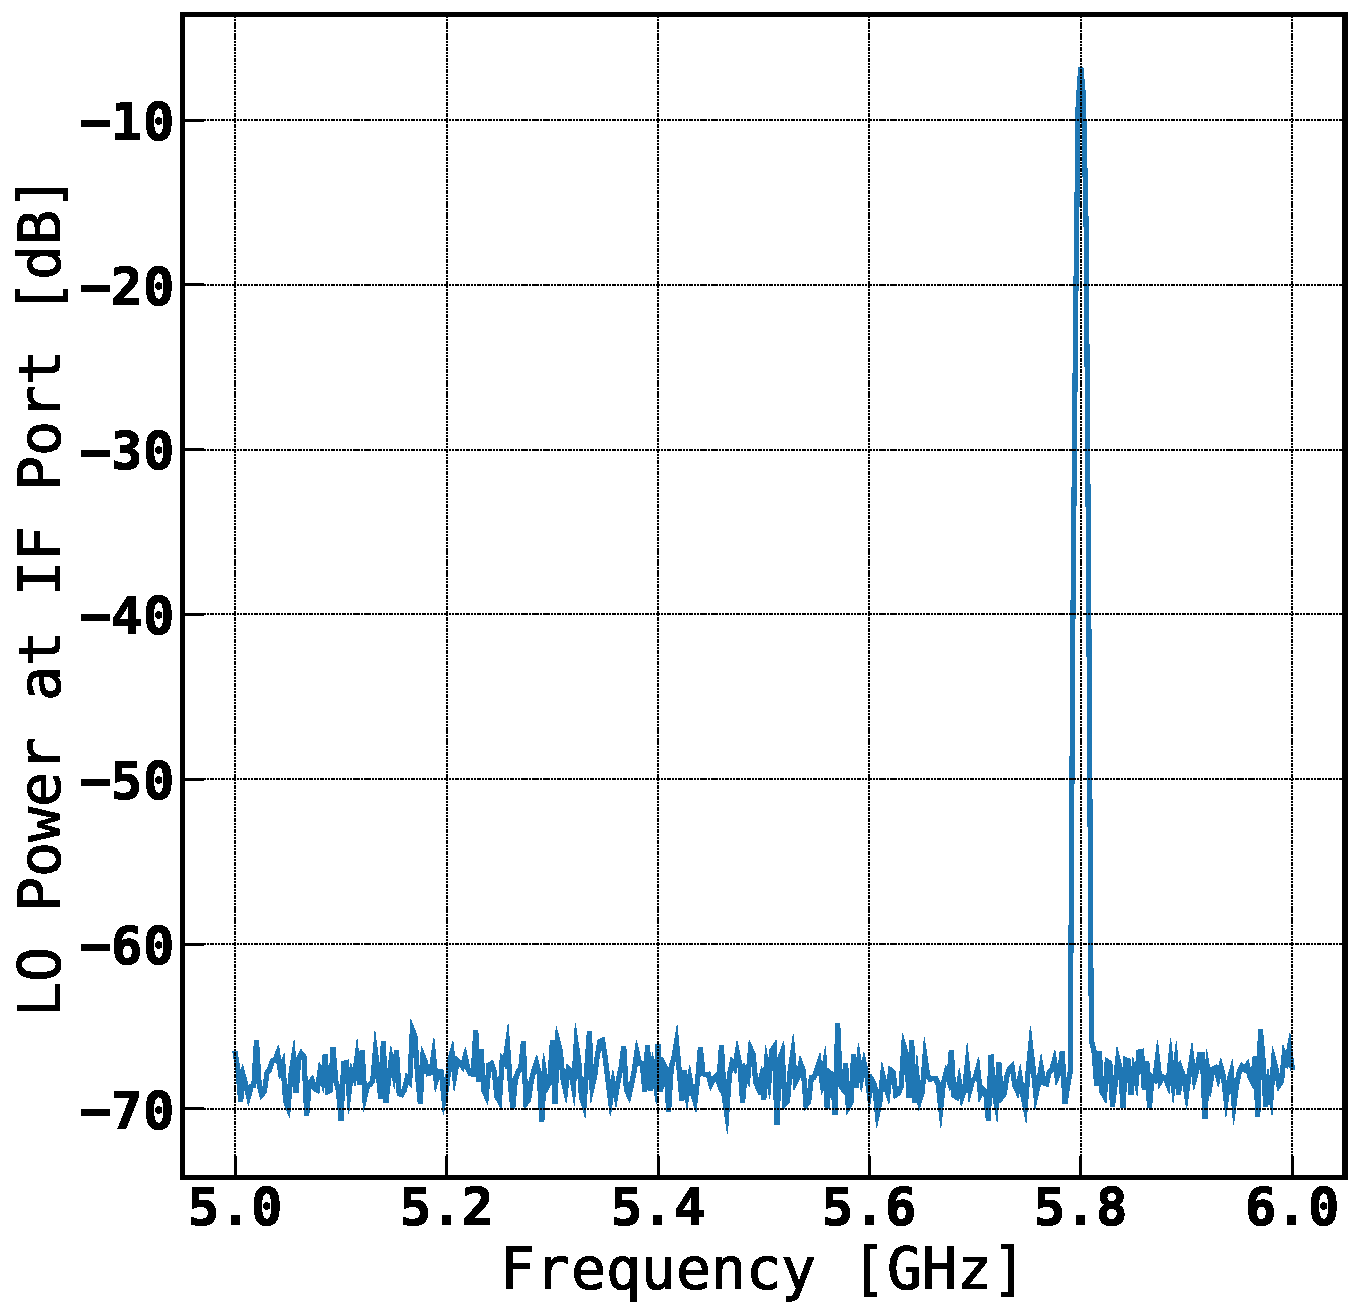
\includegraphics[scale=0.35]{Mixer_LO.pdf}
    \caption{LO isolation at the RF port}
    \label{fig:mixerLO}
\end{figure}

\begin{figure}[!htbp]
    \centering
    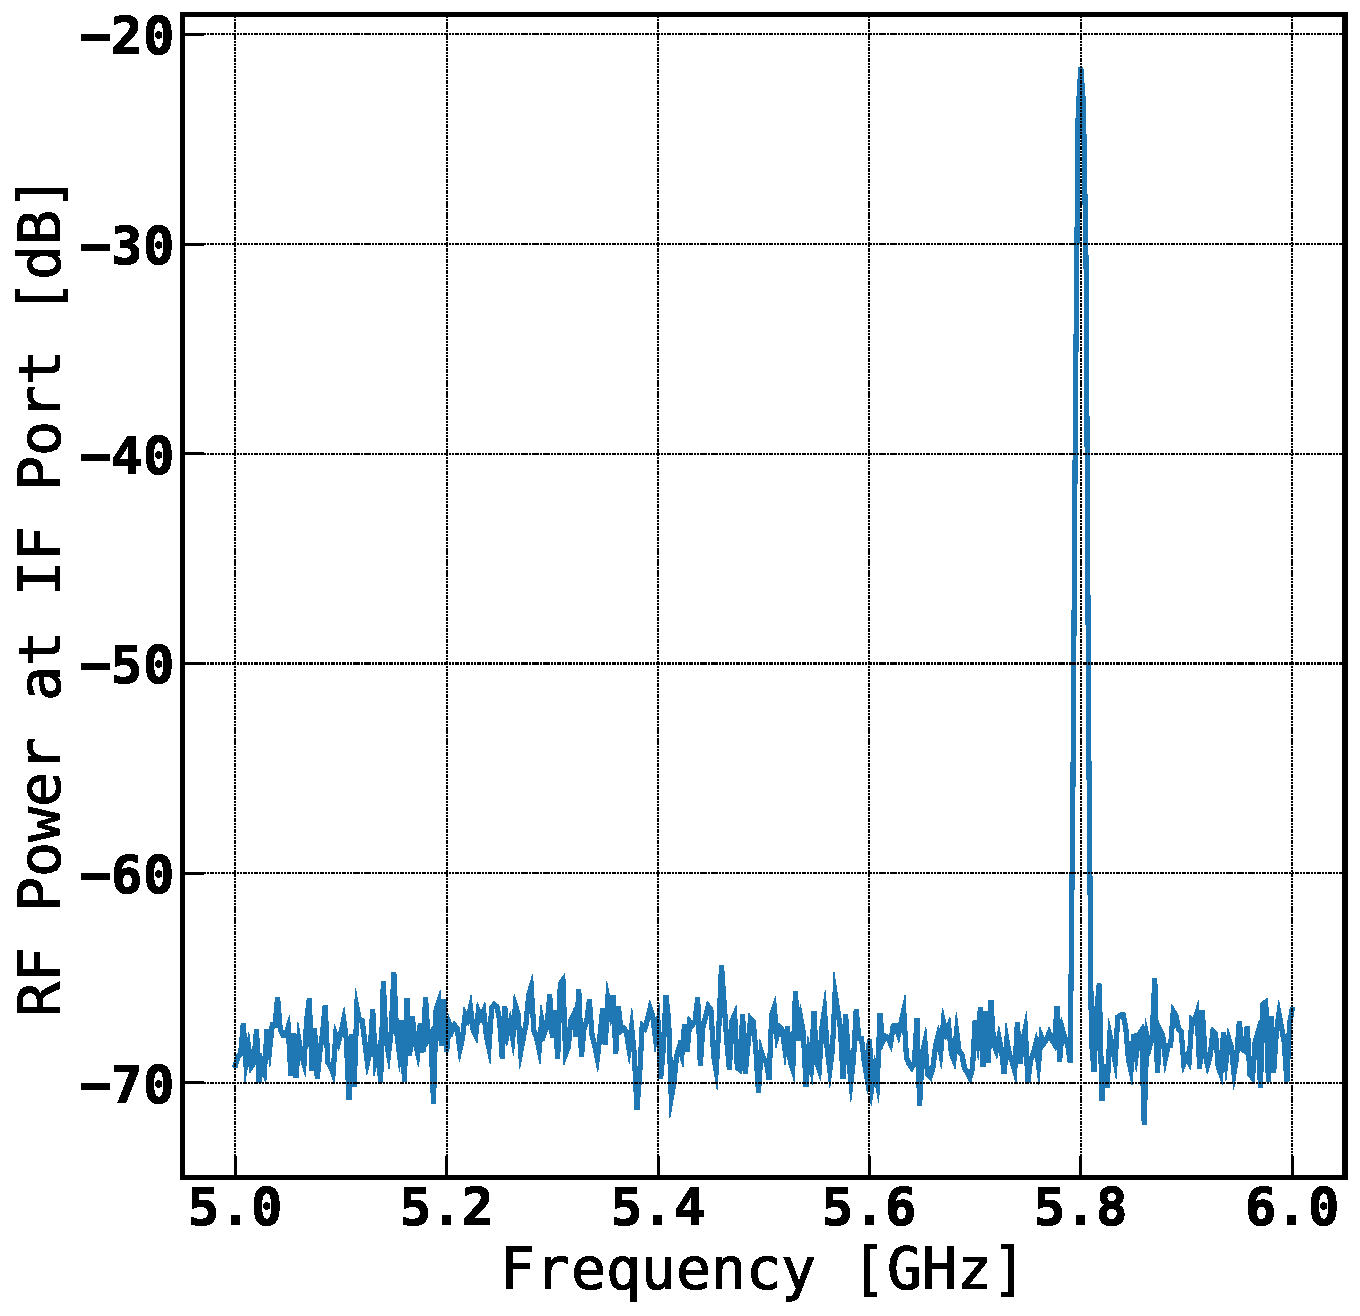
\includegraphics[scale=0.35]{Mixer_RF.pdf}
    \caption{LO isolation at the RF port}
    \label{fig:mixerRF}
\end{figure}


\begin{figure}[!htbp]
    \centering
    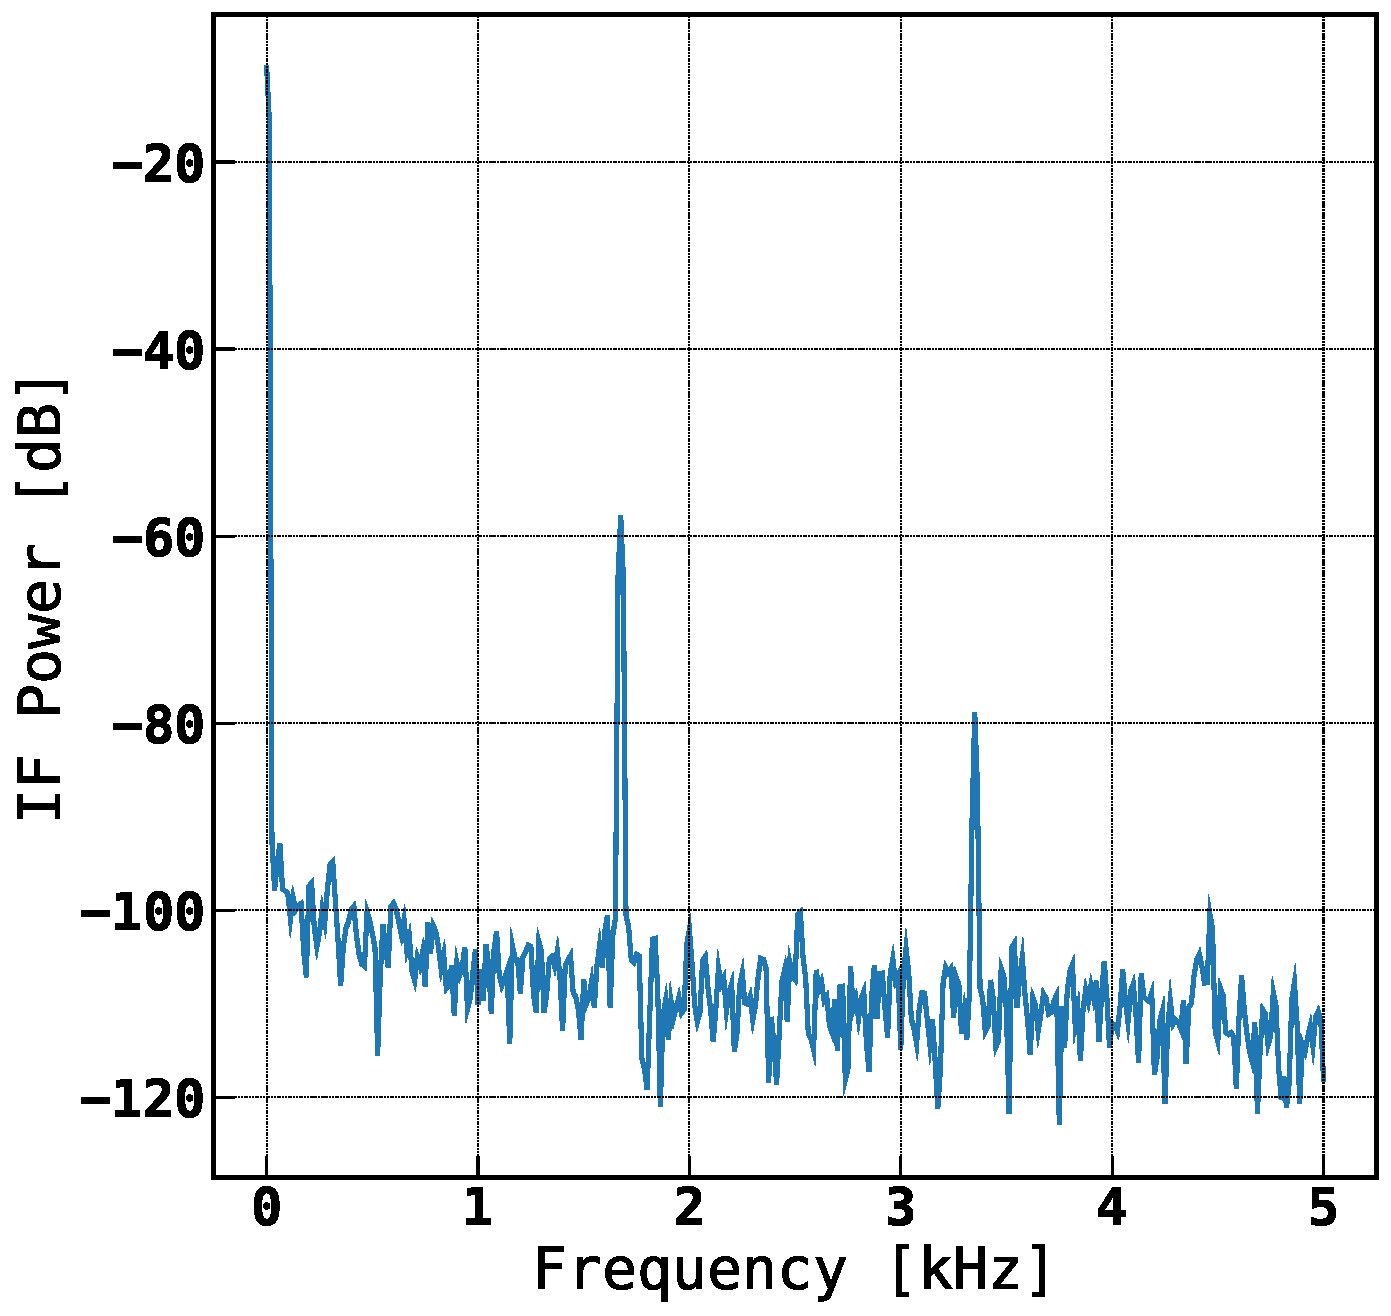
\includegraphics[scale=0.35]{Mixer_1K.pdf}
    \caption{Conversion Loss High}
    \label{fig:mixer1}
\end{figure}

\begin{figure}[!htbp]
    \centering
    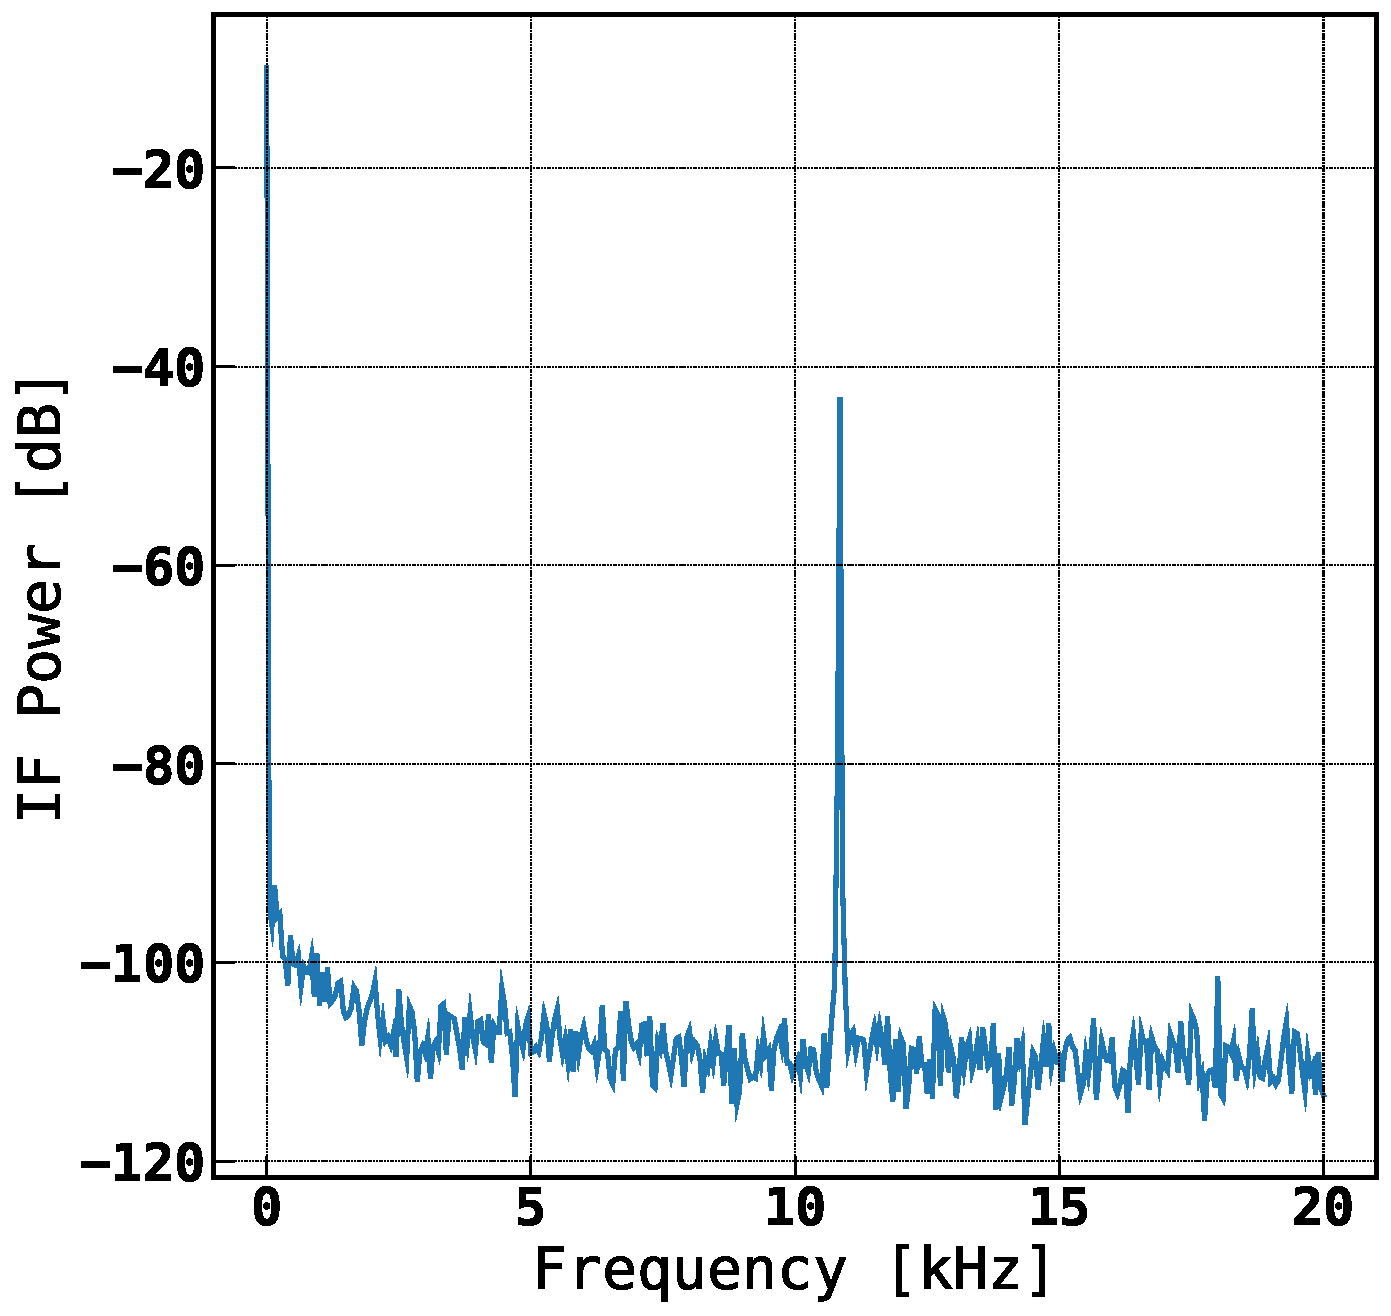
\includegraphics[scale=0.35]{Mixer_10K.pdf}
    \caption{Conversion Loss Low}
    \label{fig:mixer10}
\end{figure}


- Measured the S parameters of the LNA + PA as well as the noise. Both biased to 3 V, 50 mA current. The simulated gains of the LNA and PA showed in figures [\ref{figLNAGain}, \ref{fig:PAGain}] respectively. For the combined amplifier, the simulated gain and noise performance shown in figure [\ref{fig:LNAGainNoise}]. Actual measured LNA + PA showed worse performance with a total gain of 22 dB and a noise temperature of about 170K. The comparison between measured and sims shown in figure [\ref{fig:LNAPAmeas}]

\begin{figure}[!htbp]
    \centering
    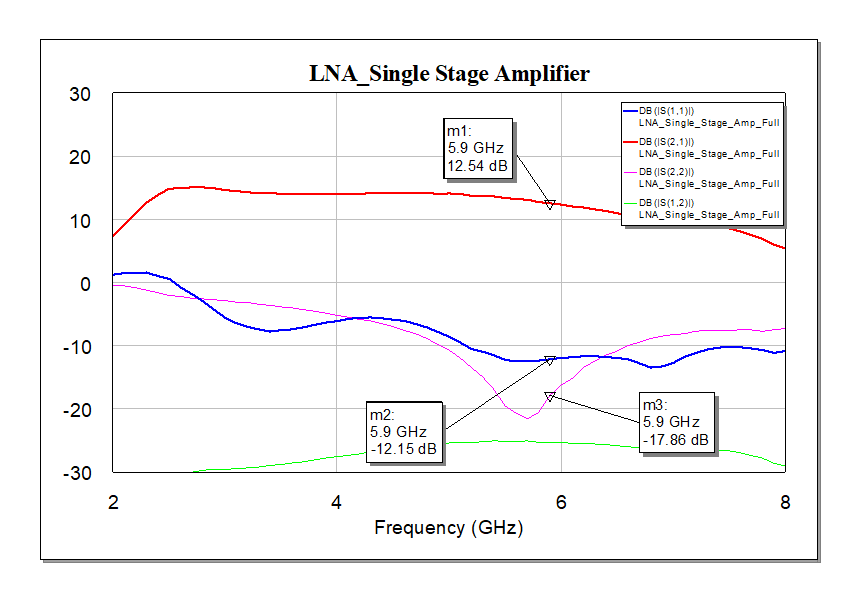
\includegraphics[scale=0.35]{LNA_Gain.png}
    \caption{Simulated gain of the LNA.}
    \label{fig:LNAGain}
\end{figure}

\begin{figure}[!htbp]
    \centering
    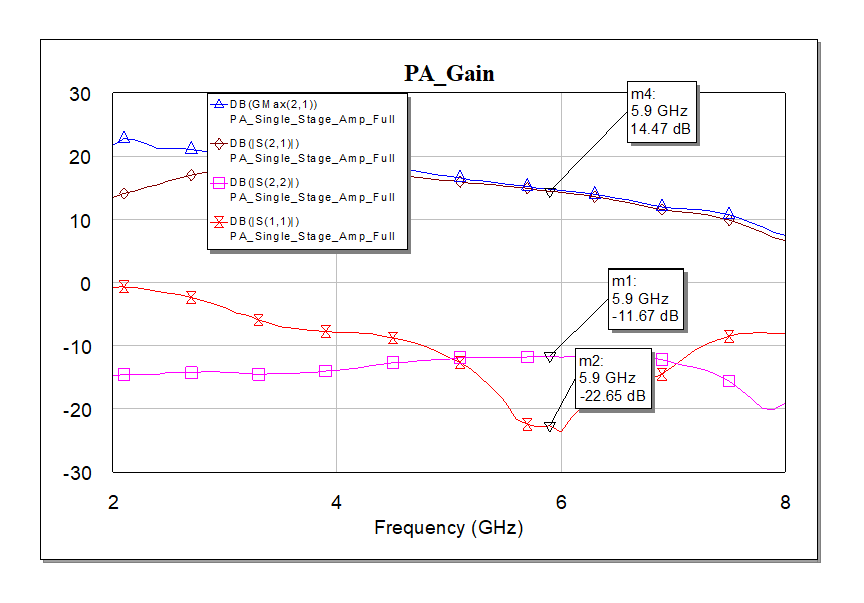
\includegraphics[scale=0.35]{PA_Gain.png}
    \caption{Simulated gain of the PA.}
    \label{fig:PAGain}
\end{figure}

\begin{figure}[!htbp]
    \centering
    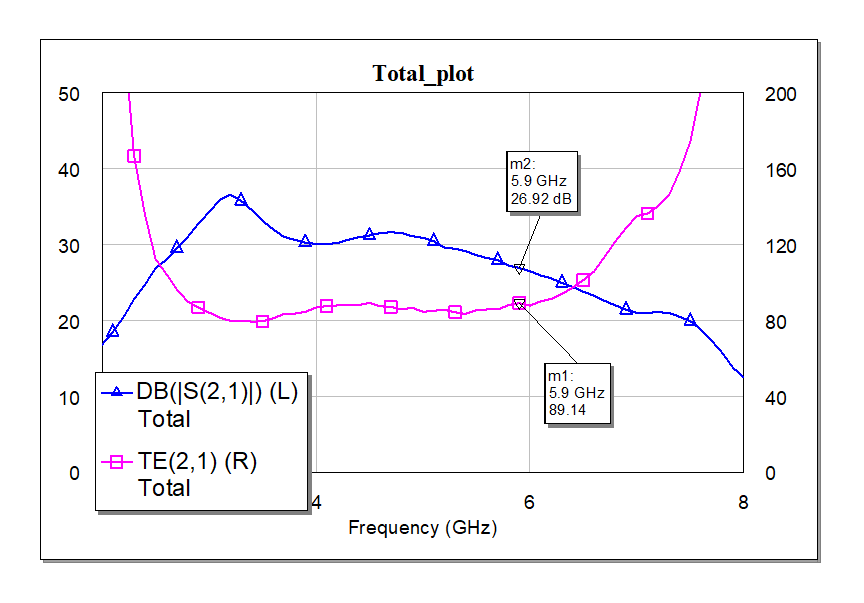
\includegraphics[scale=0.35]{LNA+PA_Gain+Noise.png}
    \caption{Noise performance of the combined LNA and PA stage.}
    \label{fig:LNAGainNoise}
\end{figure}

\begin{figure}[!htbp]
    \centering
    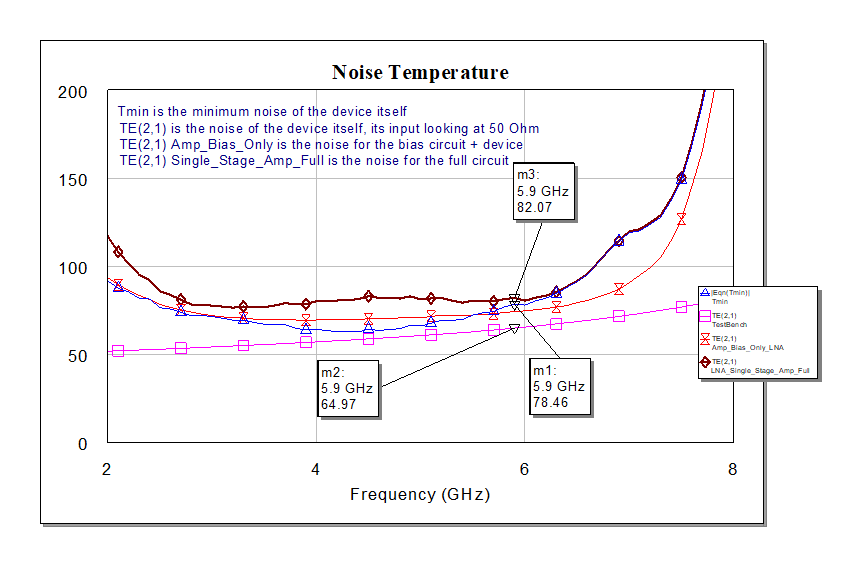
\includegraphics[scale=0.35]{LNA_Noise_Temperature.png}
    \caption{Simulated noise performance of the LNA. }
    \label{fig:LNANoiseTemp}
\end{figure}



\begin{figure}[!htbp]
    \centering
    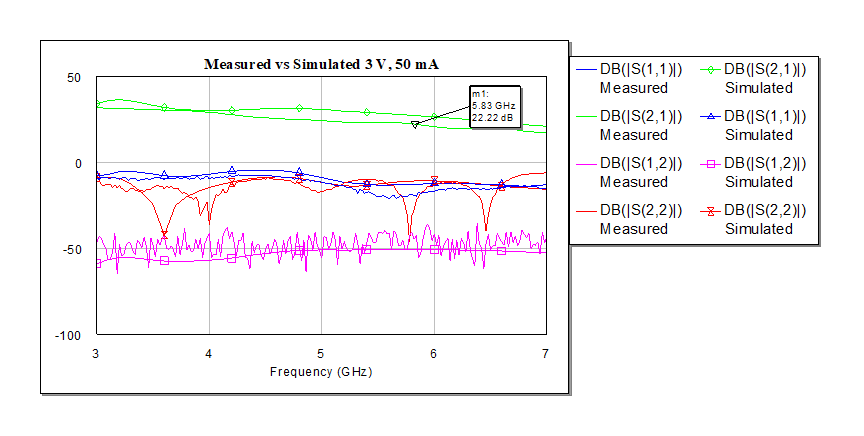
\includegraphics[scale=0.35]{LNA+PA_Measured.png}
    \caption{A comparison of the simulated vs measured parameters of the amplifiers.}
    \label{fig:LNAPAmeas}
\end{figure}


\begin{figure}[!htbp]
    \centering
    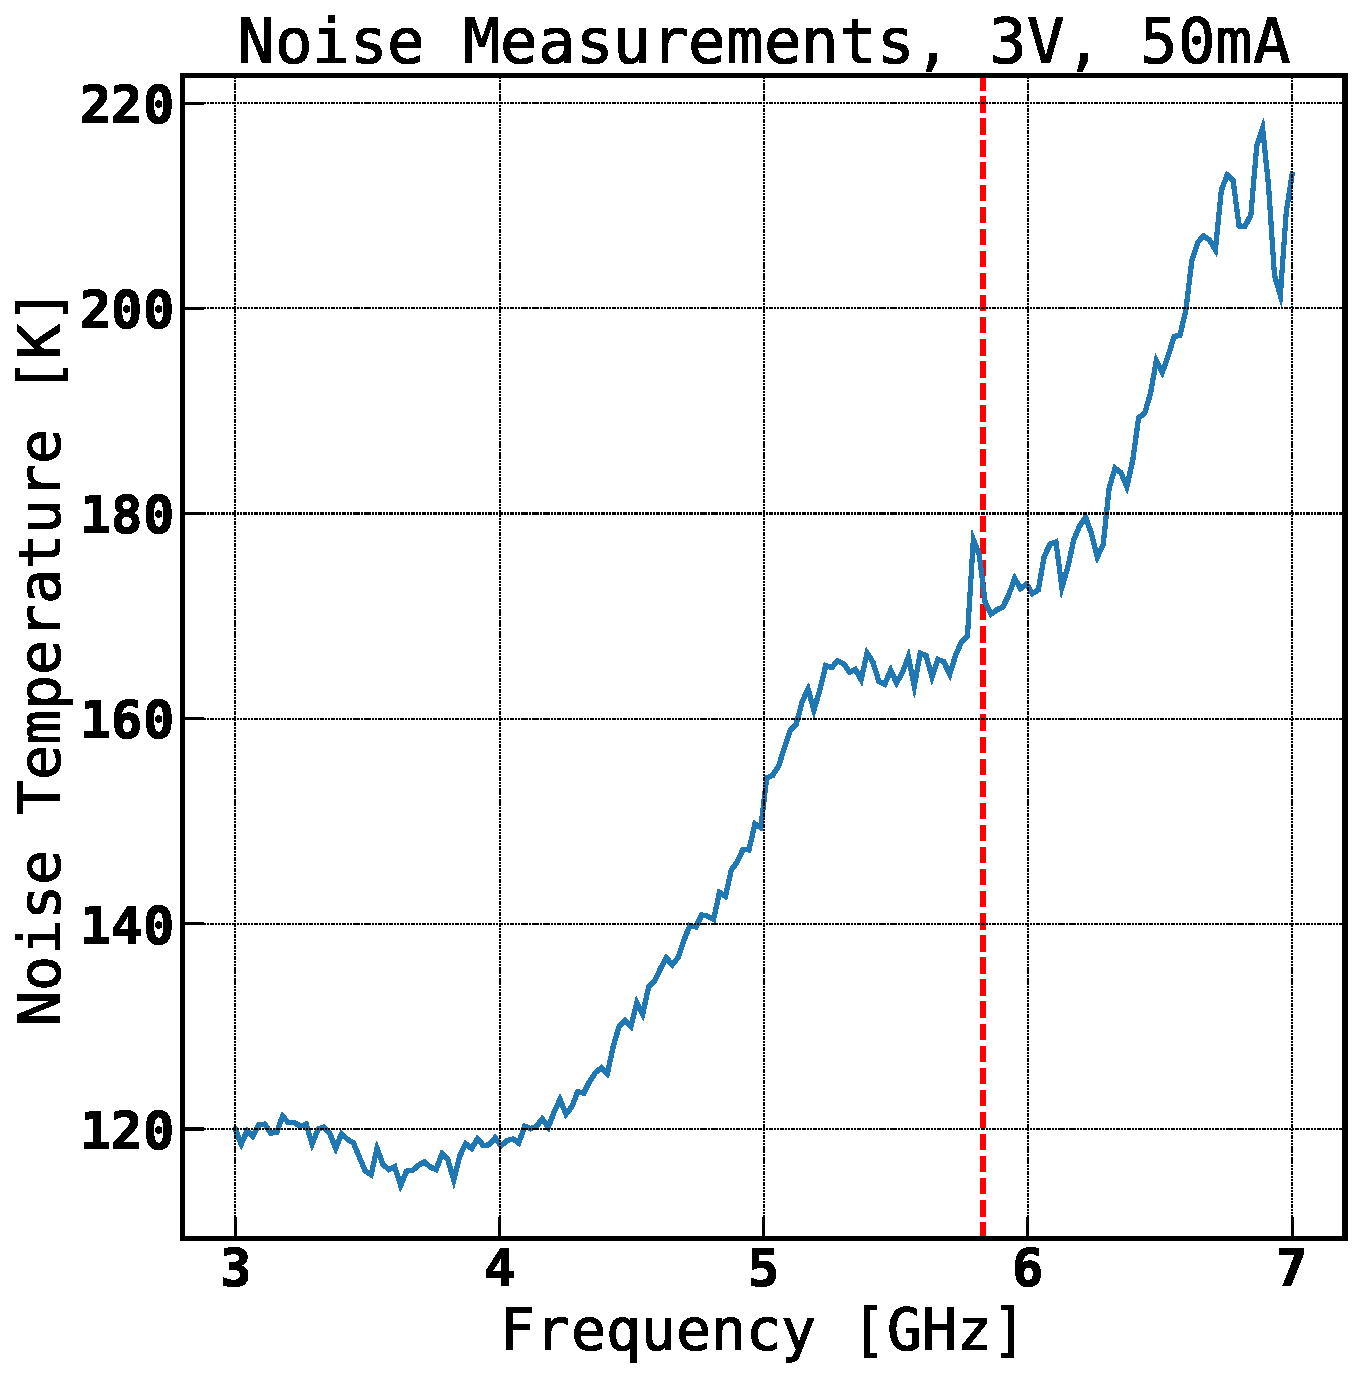
\includegraphics[scale=0.35]{LNA_PA_noisemeas.pdf}
    \caption{A comparison of the simulated vs measured noise temperature of the amplifiers.}
    \label{fig:LNAPAnoise}
\end{figure}
- For the Wilkinson, similarly had 1 higher dB loss in the transmit side and about expected in the mixer side. Comparison between meas and sims shown in figure [\ref{fig:AsWilksimMeas}].



\begin{figure}[!htbp]
    \centering
    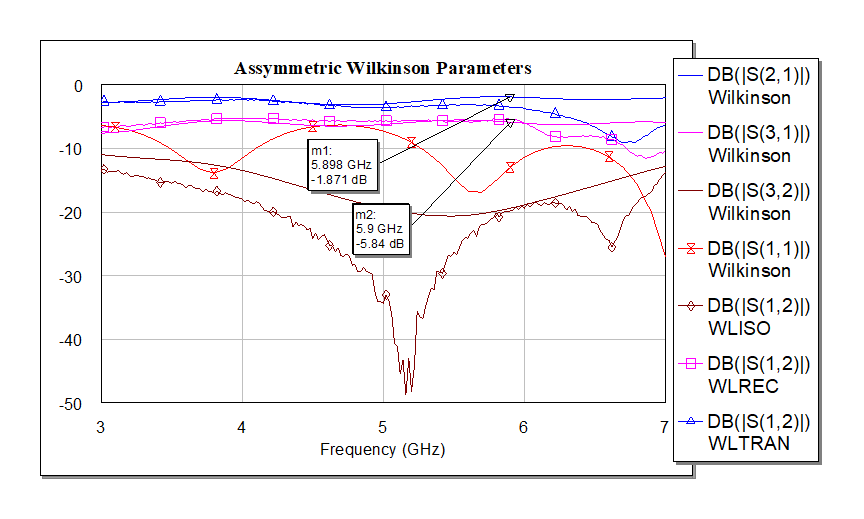
\includegraphics[scale=0.35]{Unbalanced_Wilkinson_Meas.png}
    \caption{Comparison of the measured vs simulated performance of the power splitter.}
    \label{fig:AsWilksimMeas}
\end{figure}

\begin{figure}[!htbp]
    \centering
    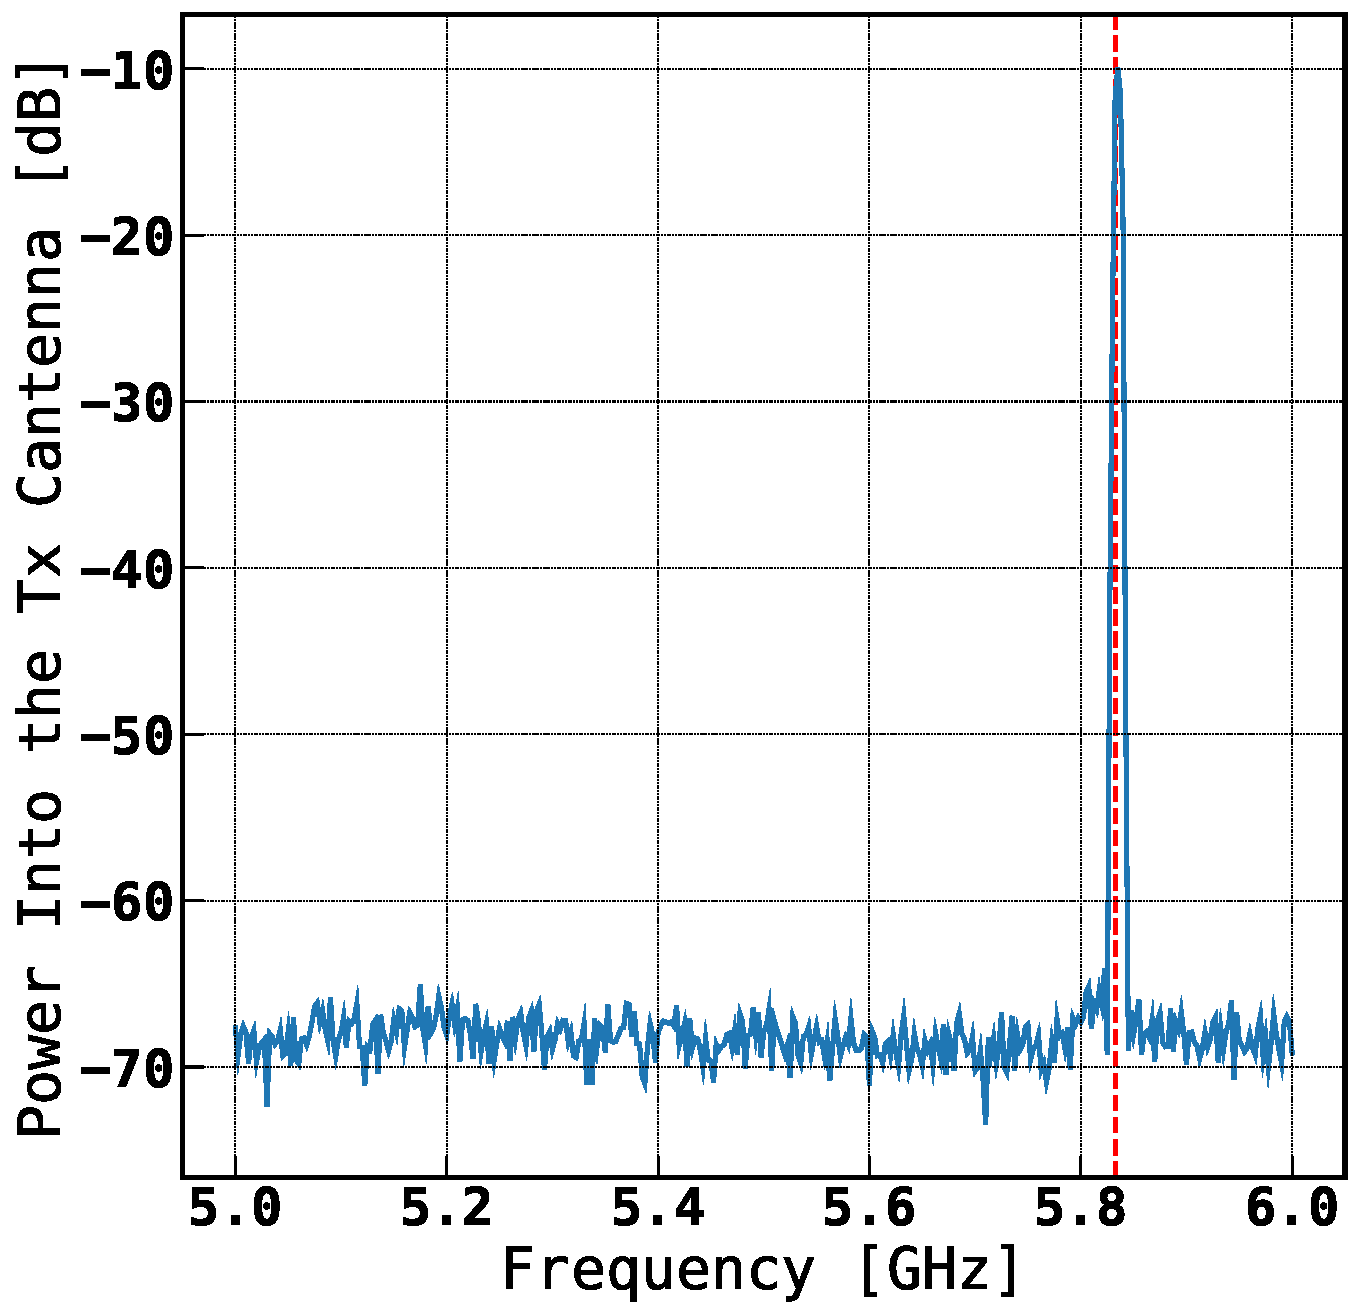
\includegraphics[scale=0.35]{Tx_Power.pdf}
    \caption{A measurement of the power split to the transmitter.}
    \label{fig:txpowersplit}
\end{figure}

\begin{figure}[!htbp]
    \centering
    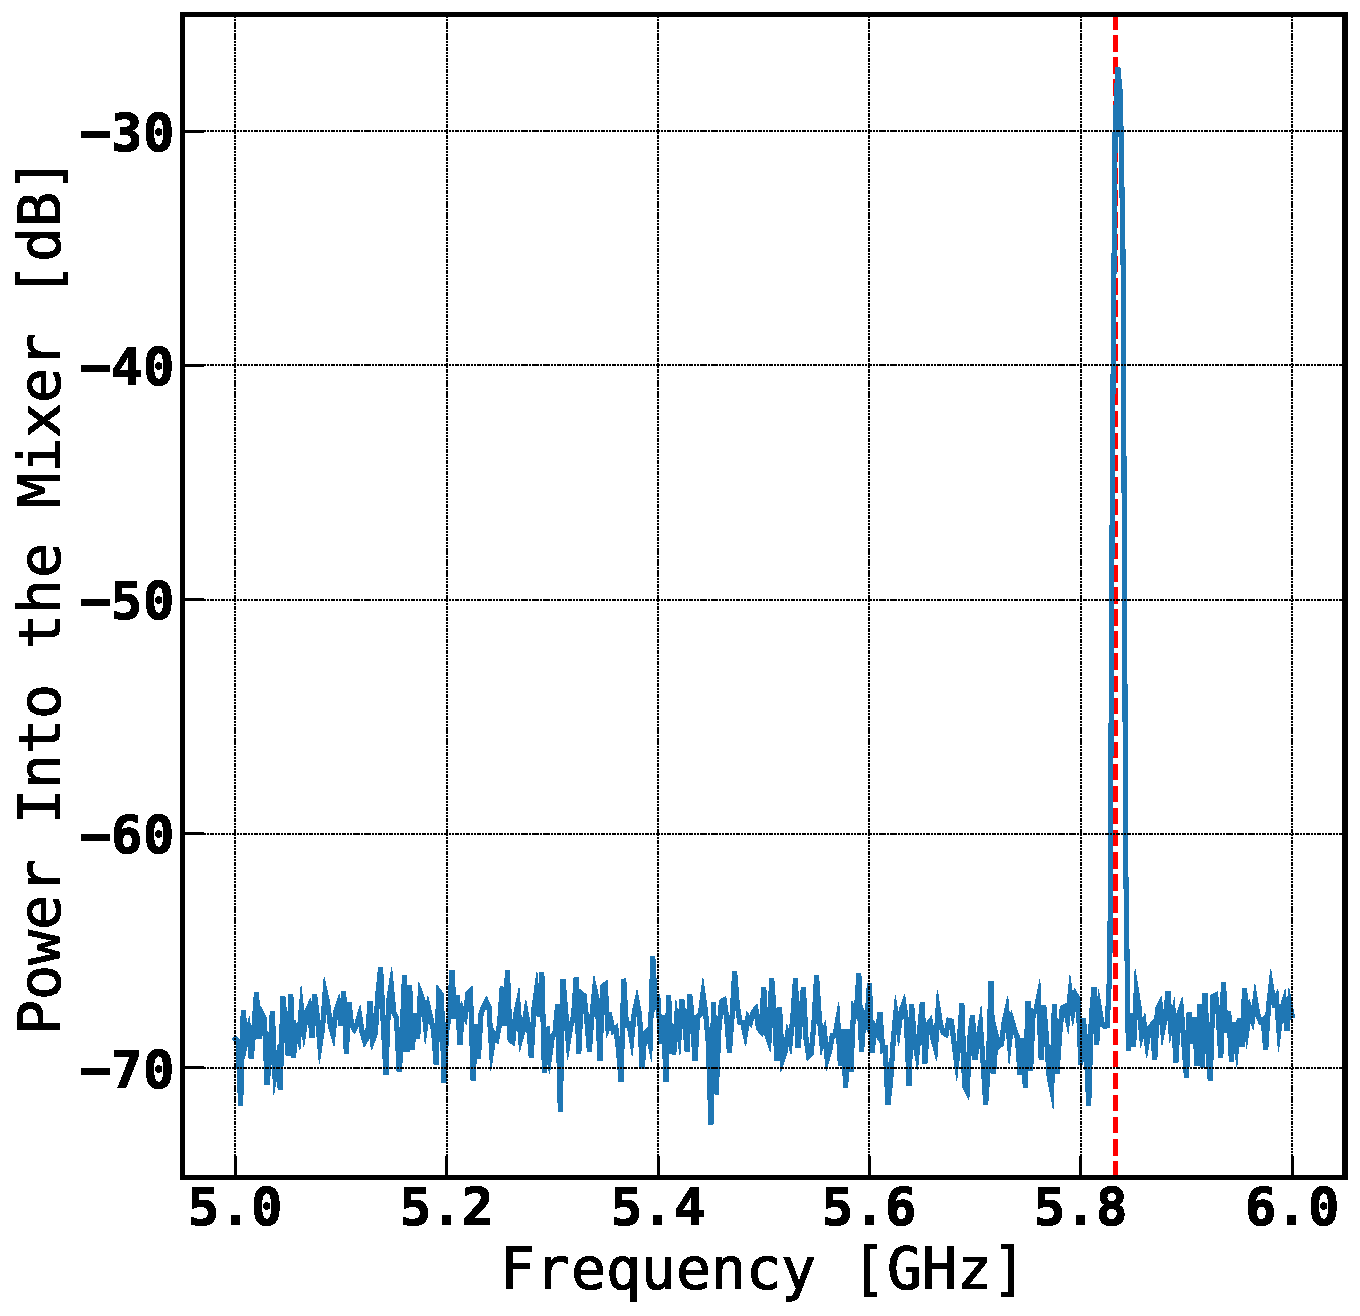
\includegraphics[scale=0.35]{Mixer_Power.pdf}
    \caption{A measurement of the power split to the Mixer.}
    \label{fig:mixpowersplit}
\end{figure}

- Tested the entire VCO and amplifier stage for the transmit side. I can't remember how it actually compared with the datasheets. Please check!! Figure [\ref{fig:VCO}]

\begin{figure}[!htbp]
    \centering
    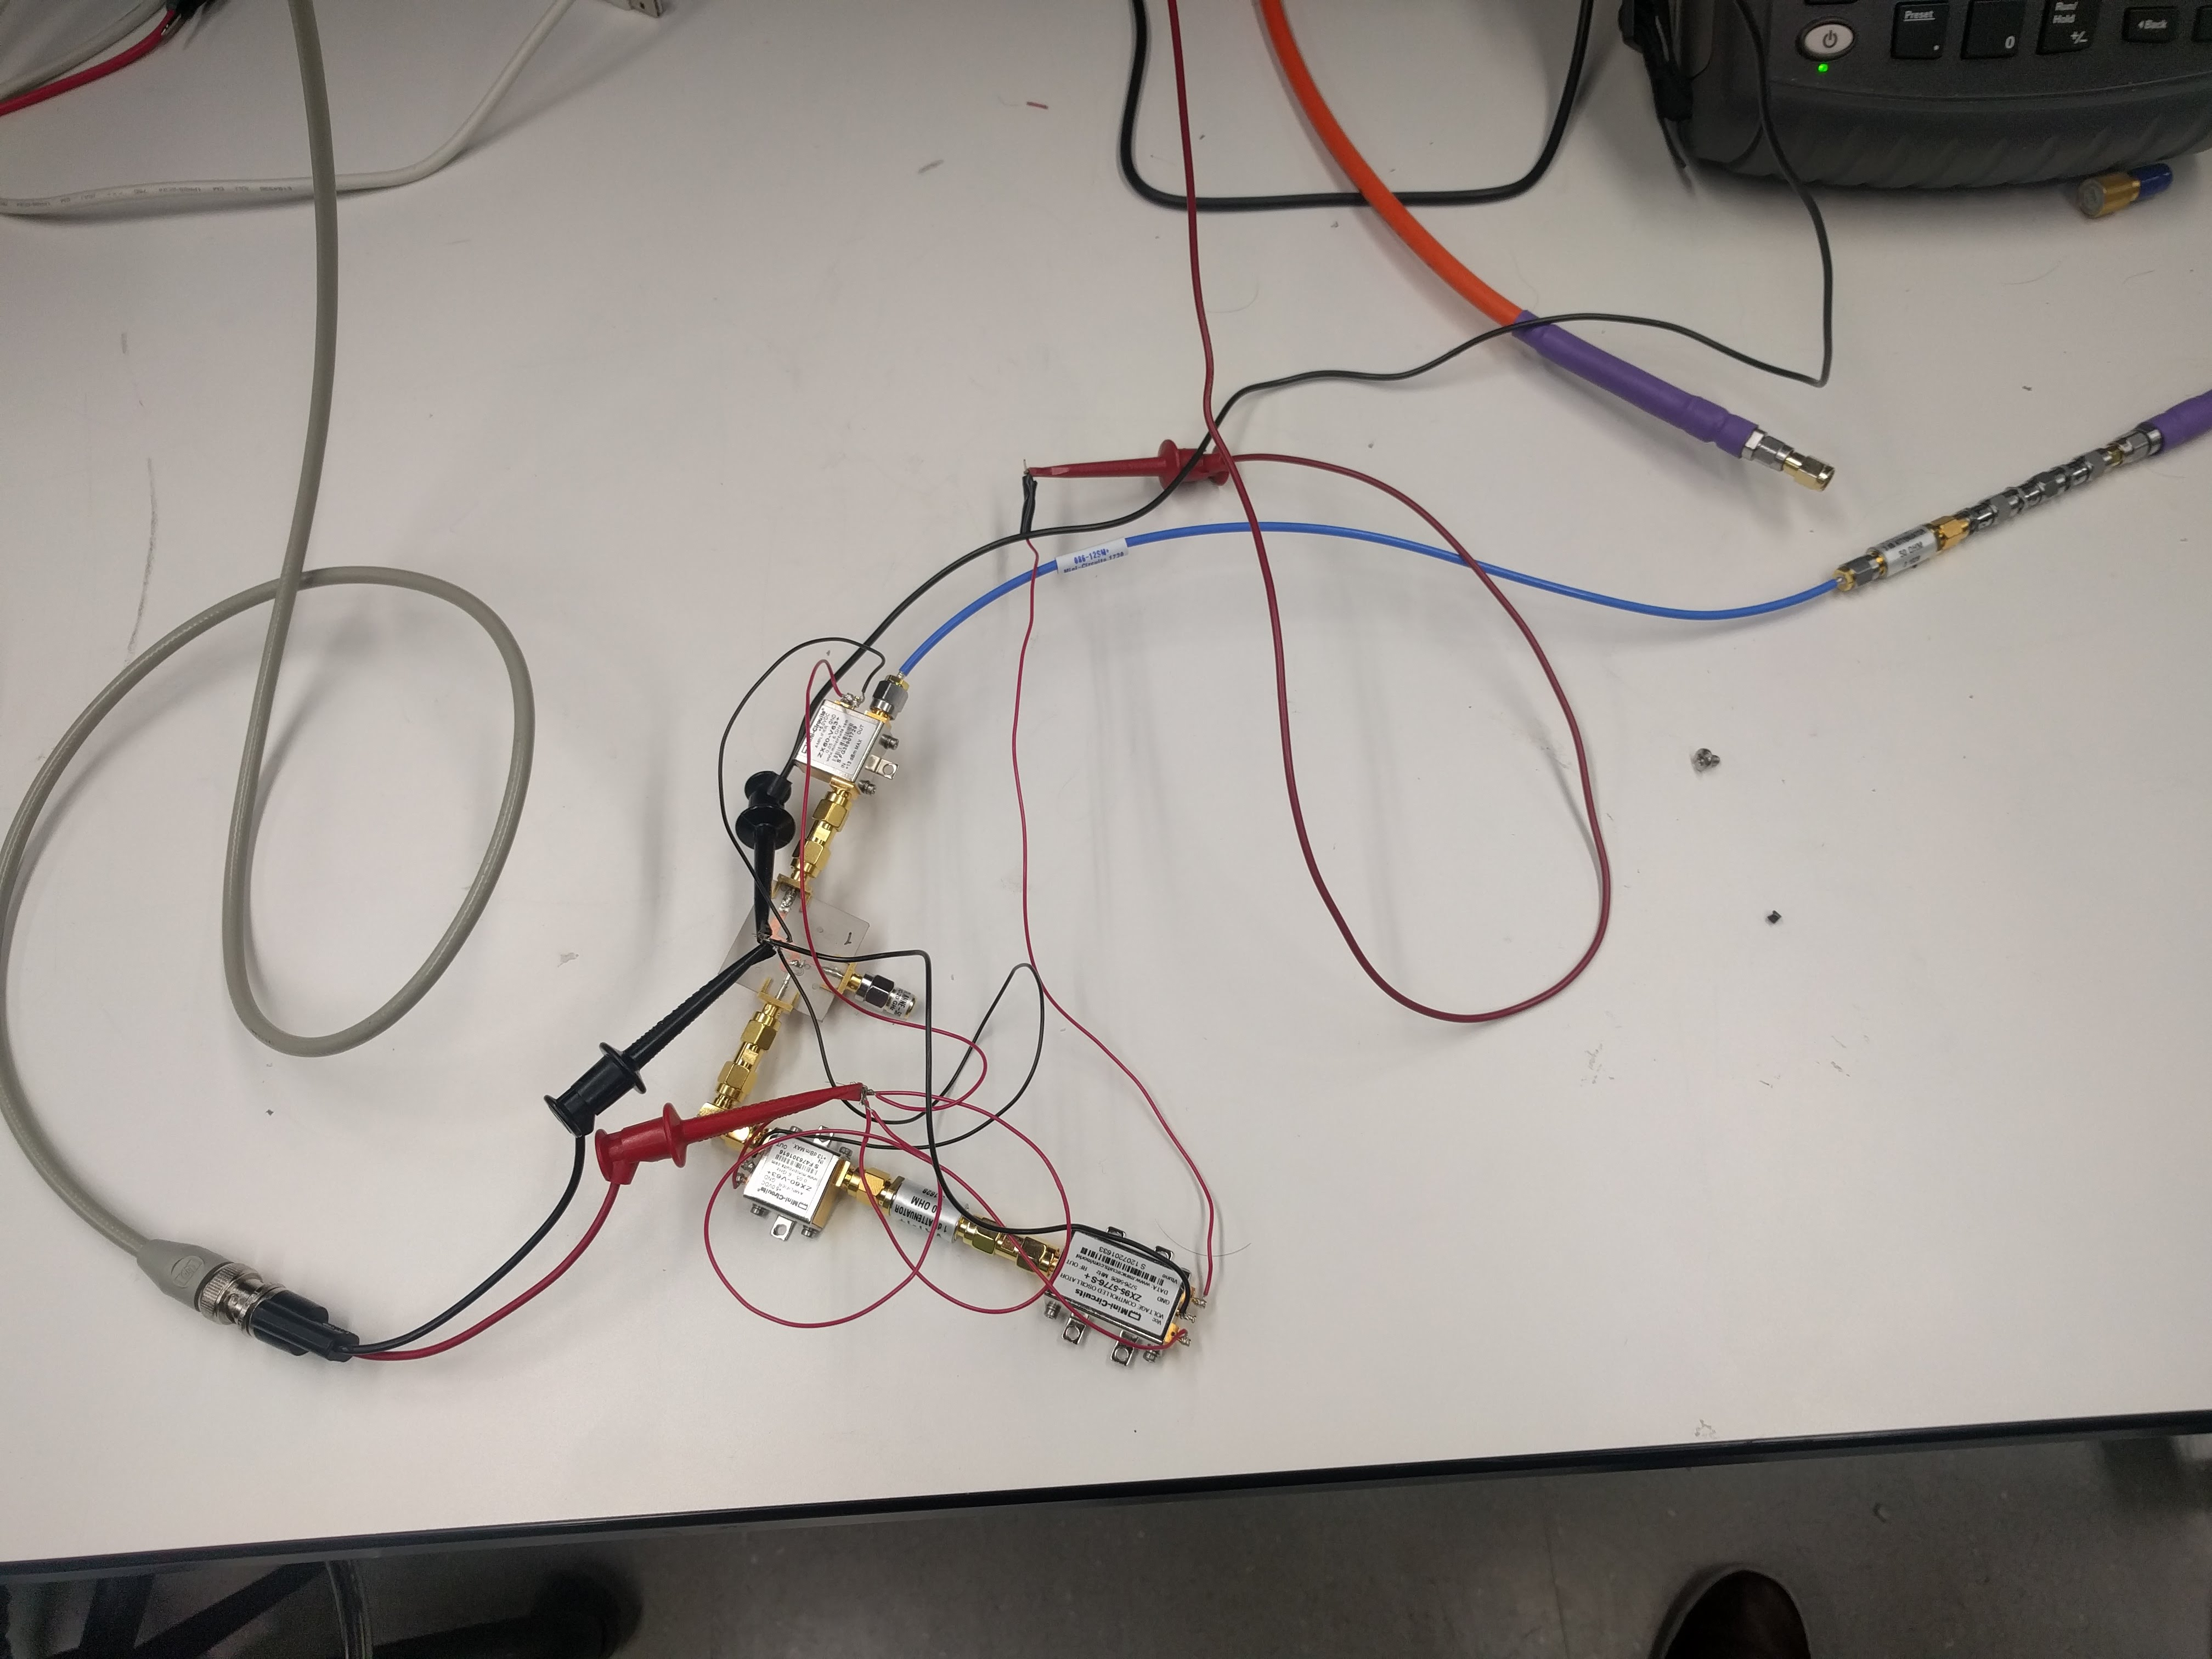
\includegraphics[scale=0.05]{VCO.jpg}
    \caption{Measuring the performance of the VCO and amplifier stage for the transmitter.}
    \label{fig:VCO}
\end{figure}

- Tested the radar board by powering it and measuring the audio signal out using an oscilloscope and using a set of speakers.

\section*{System Level Testing}

- Trouble with recording audio

- Doing the walk test

- Ensuring all the connections were tight using the torque wrench

- Continuity tests using a multimeter

- Figuring out how to bias the amplifiers. Minwo's clever solution


\section*{Final Results}


\section*{Summary}


\end{document}